%% FEUP THESIS STYLE for LaTeX2e
%% how to use feupteses (English version)
%%
%% FEUP, JCL & JCF, 31 July 2012
%%
%% PLEASE send improvements to jlopes at fe.up.pt and to jcf at fe.up.pt
%%

%%========================================
%% Commands: pdflatex tese
%%           bibtex tese
%%           makeindex tese (only if creating an index) 
%%           pdflatex tese
%% Alternative:
%%          latexmk -pdf tese.tex
%%========================================

\documentclass[11pt,a4paper,twoside,openright]{report}

%% For iso-8859-1 (latin1), comment next line and uncomment the second line
\usepackage[utf8]{inputenc}
%\usepackage[latin1]{inputenc}

%% English version

%% MIEIC options
%\usepackage[mieic]{feupteses}
%\usepackage[mieic,juri]{feupteses}
\usepackage[mieic,final]{feupteses}
%\usepackage[mieic,final,onpaper]{feupteses}

%% Additional options for feupteses.sty: 
%% - onpaper: links are not shown (for paper versions)
%% - backrefs: include back references from bibliography to citation place

%% Uncomment the next lines if side by side graphics used
%\usepackage[lofdepth,lotdepth]{subfig}
%\usepackage{graphicx}
%\usepackage{float}

%% Include color package
\usepackage{color}
\definecolor{cloudwhite}{cmyk}{0,0,0,0.025}

%% Include source-code listings package
\usepackage{listings}
\lstset{ %
 language=C,                        % choose the language of the code
 basicstyle=\footnotesize\ttfamily,
 keywordstyle=\bfseries,
 numbers=left,                      % where to put the line-numbers
 numberstyle=\scriptsize\texttt,    % the size of the fonts that are used for the line-numbers
 stepnumber=1,                      % the step between two line-numbers. If it's 1 each line will be numbered
 numbersep=8pt,                     % how far the line-numbers are from the code
 frame=tb,
 float=htb,
 aboveskip=8mm,
 belowskip=4mm,
 backgroundcolor=\color{cloudwhite},
 showspaces=false,                  % show spaces adding particular underscores
 showstringspaces=false,            % underline spaces within strings
 showtabs=false,                    % show tabs within strings adding particular underscores
 tabsize=2,	                    % sets default tabsize to 2 spaces
 captionpos=b,                      % sets the caption-position to bottom
 breaklines=true,                   % sets automatic line breaking
 breakatwhitespace=false,           % sets if automatic breaks should only happen at whitespace
 escapeinside={\%*}{*)},            % if you want to add a comment within your code
 morekeywords={*,var,template,new}  % if you want to add more keywords to the set
}

%% Uncomment to create an index (at the end of the document)
%\makeindex

%% Path to the figures directory
%% TIP: use folder ``figures'' to keep all your figures
\graphicspath{{figures/}}

%%----------------------------------------
%% TIP: if you want to define more macros, use an external file to keep them
%some macro definitions

% For footnotes to work in tables:
\usepackage{footnote}
\makesavenoteenv{table}
\makesavenoteenv{tabular}

% format
\newcommand{\class}[1]{{\normalfont\slshape #1\/}}

% entities
\newcommand{\Feup}{Faculdade de Engenharia da Universidade do Porto}

\newcommand{\svg}{\class{SVG}}
\newcommand{\scada}{\class{SCADA}}
\newcommand{\scadadms}{\class{SCADA/DMS}}

%% For notes:
\usepackage{todonotes}
\newcommand\miguel[1]{\todo[color=green!40]{\small} #1}

% References
\usepackage{csquotes}
\usepackage[style=trad-alpha, backend=biber, maxcitenames=2]{biblatex}
\addbibresource{library.bib}
\addbibresource{web.bib}

\newcommand { \PrintBibliographyBiblatex }
{%
	\renewcommand{\bibname}{References}%
	\cleardoublepage%
	\phantomsection%
	\addcontentsline{toc}{chapter}{References}%
	\begin{singlespace}
		\printbibliography
	\end{singlespace}
}

% Definitions:
\usepackage{amsmath,amssymb}
\DeclareMathAlphabet{\mathcal}{OMS}{cmsy}{m}{n}
\newtheorem{definition}{Definition}[section]

\usepackage{float} % floating elements
\usepackage{booktabs} % tables
\usepackage{multirow} % For the tables

% For floats to not appear after
\usepackage{placeins}

\let\Oldsection\section
\renewcommand{\section}{\FloatBarrier\Oldsection}

\let\Oldsubsection\subsection
\renewcommand{\subsection}{\FloatBarrier\Oldsubsection}

\let\Oldsubsubsection\subsubsection
\renewcommand{\subsubsection}{\FloatBarrier\Oldsubsubsection}
%%----------------------------------------

%%========================================
%% Start of document
%%========================================
\begin{document}

%%----------------------------------------
%% Information about the work
%%----------------------------------------
\title{Using Stacked Generalization for Anomaly Detection}
\author{Miguel Oliveira Sandim}

%% Uncomment next line for date of submission
\thesisdate{September 19, 2017}

%%Uncomment next line for copyright text if used
%\copyrightnotice{Name of the Author, 2008}

\supervisor{Supervisor}{Carlos Soares (Ph.D.)}
\supervisor{Co-Supervisor}{Bernhard Pfahringer (Ph.D.)}

%% Uncomment next line if necessary
%\supervisor{Second Supervisor}{Name of the Supervisor}

%% Uncomment committee stuff in the final version if used
\committeetext{Approved in oral examination by the committee:}
\committeemember{Chair}{Prof. Dr. Luís Filipe Teixeira}
\committeemember{External Examiner}{Prof. Dr. Paulo Cortez}
\committeemember{Supervisor}{Prof. Dr. Carlos Soares}
%\signature

%% Specify cover logo (in folder ``figures'')
\logo{uporto-feup.pdf}

%% Uncomment next line for additional text  below the author's name (front page)
%\additionalfronttext{Preparação da Dissertação}

%%----------------------------------------
%% Preliminary materials
%%----------------------------------------

% remove unnecssary \include{} commands
\begin{Prolog}
  \chapter*{Abstract}

Anomaly Detection is an important research topic nowadays, in which the intention is to find patterns in data that do not conform to expected behavior. 
This concept is applicable in a large number of different domains and contexts, such as intrusion detection, fraud detection, medical research and social network analysis.

Techniques that have been addressed within this topic are diverse, based on different assumptions about how anomalies manifest themselves within the data and can have different outputs (i.e. a numeric score or a labeled classification).
Because of this heterogeneity, every technique is specialized in specific characteristics of the data and may only provide a limited insight on what anomalies exist in a given dataset.

Ensemble Learning is process that tries to incorporate the opinions of different learners in order to make a more pondered decision.
This process has been successfully applied in the past to supervised and unsupervised learning problems and improvements in performance have been empirically observed.
Stacked Generalization is one of these methods, in which a learning algorithm is used to combine the different learners.

Several state of the art Anomaly Detection techniques and datasets used throughout the literature were used in this work, which was divided in two different research studies.
The first study focused on the performance and diversity of the Anomaly Detection techniques selected, while the second one focused on the application of Stacked Generalization to the techniques selected.

The first study gathered some evidence that most Anomaly Detection techniques used are \textit{accurate} and \textit{diverse}, therefore allowing the conditions for Stacked Generalization to be applied to this case.
The second study concluded that the Stacked Generalization method guaranteed higher performance than the best Anomaly Detection technique on more than half of the datasets used.
Replacing the Stacked Generalization method's meta-classifier with a simpler Majority Voting method improved the performance on even more datasets.

Possible future work could include gathering datasets with more observations and using a higher variety of Anomaly Detection techniques. This last point would likely require some implementation work, since most of the techniques referred in the literature are not implemented on general purpose programming languages.

\chapter*{Resumo}

Deteção de Anomalias é uma área de investigação importante hoje em dia, na qual a intenção é encontrar padrões em dados que não estejam de acordo com o comportamento esperado.
Este conceito é aplicável a um grande número de diferentes domínios e contextos, como deteção de intrusões, deteção de fraude, investigação médica e análise de redes sociais.

As técnicas que têm sido utilizadas nesta área são diversas, baseadas em diferentes assunções sobre como as anomalias se manifestam nos dados e podem ter diferentes resultados (uma pontuação numérica ou uma classificação). Devido a esta heterogeneidade, cada técnica é especializada em características específicas dos dados e pode apenas fornecer uma visão limitada sobre as anomalias que existem num conjunto de dados específico.

\textit{Ensemble Learning} é um processo que tenta incorporar as opiniões de diferentes algoritmos de modo a potenciar uma decisão mais ponderada.
Este processo tem sido aplicado com sucesso em problemas de aprendizagem supervisionada e não-supervisionada e melhorias na performance foram observadas empiricamente.
\textit{Stacked Generalization} é um destes métodos, no qual um algoritmo de aprendizagem é usado para combinar as opiniões de diferentes algoritmos.

Várias técnicas do estado de arte de Deteção de Anomalias e conjuntos de dados usados na literatura foram usados neste trabalho, que foi dividido em dois diferentes estudos de investigação.
O primeiro estudo focou-se na performance e diversidade das técnicas de Deteção de Anomalias selecionadas, enquanto o segundo focou-se na aplicação de \textit{Stacked Generalization} nas técnicas selecionadas.

O primeiro estudo revelou algumas evidências de que a maioria das técnicas de Deteção de Anomalias usadas é \textit{exata} e \textit{diversa}, garantindo as condições para que o \textit{Stacked Generalization} seja aplicado a este caso.
O segundo estudo concluiu que o método \textit{Stacked Generalization} garantiu uma maior performance que a melhor técnica de Deteção de Anomalias em mais de metade dos conjuntos de dados usados.
Substituindo o meta-classificador do método \textit{Stacked Generalization} por um método \textit{Majority Voting} simples melhorou a performance em ainda mais conjuntos de dados.

Possível trabalho futuro inclui reunir conjuntos de dados com mais observações e usar uma variedade maior de técnicas de Deteção de Anomalias. Este último ponto provavelmente requererá algum trabalho de implementação, dado que a maior das técnicas referidas na literatura não estão implementadas nas linguagens de programação comuns.
 % the abstract
  \chapter*{Acknowledgements}

First of all I would like to thank my supervisors, Dr. Carlos Soares and Dr. Bernhard Pfahringer, for guiding me throughout this dissertation topic and pointing me in the right directions when developing this research work.

I would like to thank Daniel for all the support given and kind words in the right moments, my family and my friends João, Ana, Paula, Luís, Susana and Raquel for all their support.
Without them, I know that I would not have been as successful as I was on my research.

Finally, I would like to thank Cláudio Sá, Tiago Cunha, Pedro Ribeiro, Fábio Pinto and Pedro Abreu from INESC TEC for their valuable insights, brainstorming sessions for this dissertation and kind availability to help me.


\vspace{10mm}
\flushleft{Miguel Oliveira Sandim}
  % the acknowledgments
  \cleardoublepage
\thispagestyle{plain}

\vspace*{8cm}

%\begin{flushright}
%   \textsl{``You should be glad that bridge fell down. \\
%           I was planning to build thirteen more to that same design''} \\
%\vspace*{1.5cm}
%           Isambard Kingdom Brunel
%\end{flushright}

%\begin{flushright}
%   \textsl{Follow your passion. \\
%   		   Stay true to yourself.\\
%   		   Never follow someone else's path unless you're in the woods \\
%   		   and you're lost and you see a path.\\
%   		   By all means, you should follow that.} \\
%\vspace*{1.5cm}
%           Ellen DeGeneres
%\end{flushright}

\begin{flushright}
   \textsl{``Your time is limited, so don't waste it living someone else's life.\\
   	Don't be trapped by dogma -- which is living with the results of other people's thinking.\\
   	Don't let the noise of others' opinions drown out your own inner voice.\\
   	And most important, have the courage to follow your heart and intuition.''} \\
\vspace*{1.5cm}
           Steve Jobs
\end{flushright}




       % initial quotation if desired
  \cleardoublepage
  \pdfbookmark[0]{Table of Contents}{contents}
  \tableofcontents
  \cleardoublepage
  \pdfbookmark[0]{List of Figures}{figures}
  \listoffigures
  \cleardoublepage
  \pdfbookmark[0]{List of Tables}{tables}
  \listoftables
  \chapter*{Abbreviations}
\chaptermark{ABBREVIATIONS}

\begin{flushleft}
\begin{tabular}{l p{0.8\linewidth}}
	
SVM & Support Vector Machine \\
LOF & Local Outlier Factor \\
COF & Connectivity-based Outlier Factor \\
ODIN & Outlier Detection using In-degree Number \\
LOCI & Location Correlation Integral \\
DBSCAN & Density-based Spatial Clustering of Applications with Noise \\
SOM & Self Organizing Maps \\
PCA & Principal Component Analysis \\
CAR & Classification Association Rules \\
EM & Expectaction-Maximization \\
CART & Classification And Regression Tree \\
NB & Naive Bayes \\
RF & Random Forest \\
MLP & Multilayer Perceptron \\
LR & Logistic Regression

%ADT      & Abstract Data Type\\
%ANDF     & Architecture-Neutral Distribution Format\\
%API      & Application Programming Interface\\
%CAD      & Computer-Aided Design\\
%CASE     & Computer-Aided Software Engineering\\
%CORBA    & Common Object Request Broker Architecture\\
%UNCOL    & UNiversal COmpiler-oriented Language\\
%Loren    & Lorem ipsum dolor sit amet, consectetuer adipiscing
%elit. Sed vehicula lorem commodo dui\\
%WWW      & \emph{World Wide Web}
\end{tabular}
\end{flushleft}

  % the list of abbreviations used
\end{Prolog}

%%----------------------------------------
%% Body
%%----------------------------------------
\StartBody

%% TIP: use a separate file for each chapter
\chapter{Introduction} \label{chap:intro}

\section*{}

Data Mining has become an important field in the modern world, given the large number of possible applications in many different domains such as marketing, medical research, computer vision, social network analysis, intrusion detection and fraud detection \cite{Aggarwal:2015:DMT:2778285}.
This diverse range of applications is also explained by the increase in the volume of data stored (thanks to trends such as the \textit{Internet of Things} \cite{atzori2010internet} and \textit{Industry 4.0} \cite{lasi2014industry}) and their easy and wide distribution.
%(made possible by platforms such as Kaggle \cite{Kaggle} and UCI \cite{UCI}).

Anomaly Detection is a very specific but significant topic in this field, given the high number of domains in which it can be applied \cite{Kandhari2009}. In fact, the problem that motivates this field is a very common one and can be easily translated into this question: given a certain amount of data, is it possible to detect observations that deviate from the normal behavior of the data?
This question can arise, e.g. in areas such as credit card fraud detection (where the deviant patterns can correspond to fraudulent transactions) or machine condition monitoring (in which the abnormal patterns can correspond to different vibration values of certain components belonging to an industrial machine, that might indicate a certain type of malfunction \cite{Langone2015}).

\section{Motivation and Goals} \label{sec:goals} 

The literature regarding Anomaly Detection techniques is very extensive and diverse, with a wide range of techniques that can have different outputs (either an \textit{anomaly score} that indicates how much of a data instance in a dataset is an \textit{anomaly}, or a label -- \textit{anomalous} or \textit{normal}), as well as different assumptions (e.g. density based techniques have different underlying assumptions than clustering based techniques).
This heterogeneity within Anomaly Detection techniques may cause different techniques to behave differently on the same dataset, which makes the task of choosing the right technique(s) for a specific domain very difficult and data-dependent.

The thesis intends to address this issue, by using several Anomaly Detection techniques at the same time and then combining their outputs into a single one.
This is the idea behind Ensemble Learning methods, which work by generating a group of models (which is designated by \textit{ensemble}) and then combining their predictions into one.
Ensemble Learning has proven to improve performance in machine learning applications such as classification, regression, time-series analysis and recommender systems \cite{Aggarwal:2013:OA:2436823}.
Ensemble Learning based solutions are also known to win various data mining competitions (the most well-known being the Netflix Prize challenge for recommender systems).
More specifically this thesis will explore a Stacked Generalization method, which consists in using an extra model that \textit{learns} the best way of combining the group of models.

%\textbf{MELHORAR, Colocar definição de Ensemble Learning estilo de votação. Examples are many: the essence of democracy where a group of people vote to make a decision, whether to choose an elected official or to decide on a new law, is in fact based on ensemble-based decision making.}

Therefore this thesis intends to answer the following main research question:

\begin{itemize}
	\item Can a Stacked Generalization method improve the performance of Anomaly Detection techniques, more specifically the performance of the best technique for a given dataset?
\end{itemize}

%\begin{itemize}
%	\item Ensemble Learning guarantees better results in regular supervised-learning problems (classification and regression -- cite paper from Regression Ensembles from Prof. João).
%	\item Anomaly/Outlier Detection is a very particular field of DM (and also very heterogenous, with several types of methods that have distinct outputs): describe the field very shortly, stating that we usually want to find ``unsual'' patterns that don't go along the normal behavior of the data: some problems can be viewed as classification problems, in which one class is very rare and distinct from the other one (the ``anomalies''.).
%	\item It's interesting to study if the good results reported throughout the academia using Ensemble methods, apply to Anomaly Detection techniques and report the gaps in the literature in this topic, trying to improve some of them.
%\end{itemize}

%Research questions:
%\begin{itemize}
%	\item Can the concept of Ensemble Learning be applied to Anomaly Detection? What are the previous works in this topic?
%	\item What are the research opportunities in this topic?
%\end{itemize}

%Apresenta a motivação e enumera os objetivos do trabalho terminando com um resumo das metodologias para a prossecução dos objetivos.

% DESCOMENTAR DPS
\section{Outline} \label{sec:outline}

This document is structured as follows:

\begin{itemize}
	\item Chapter~\ref{chap:anomaly} reports the current state-of-the-art in Anomaly Detection, by presenting a definition for this field and techniques used;
	
	\item Chapter~\ref{chap:ensemble} describes the concepts of Ensemble Learning and Stacked Generalization along with examples of techniques and applications in the context of Anomaly Detection;
	
	\item Chapter~\ref{chap:meth} presents the methodology followed throughout the experimental research of this dissertation;
	
	\item Chapter~\ref{chap:resul} summarizes the main results and findings of the application of the experimental methodology proposed in the previous chapter;
	
	\item Chapter~\ref{chap:conc} closes this dissertation by summarizing the results gathered in the context of the field, the main contributions of this work and possible future work topics.
\end{itemize}


%Chapter \textbf{METER CAPITULO} finalizes this document with preliminary conclusions for this thesis work and planning for the future work to be carried out.

%Para além da introdução, esta dissertação contém mais x capítulos.
%No capítulo~\ref{chap:sota}, é descrito o estado da arte e são
%apresentados trabalhos relacionados. 
%\todoline{Complete the document structure.}
%No capítulo~\ref{chap:chap3}, ipsum dolor sit amet, consectetuer
%adipiscing elit.
%No capítulo~\ref{chap:chap4} praesent sit amet sem. 
%No capítulo~\ref{chap:concl}  posuere, ante non tristique
%consectetuer, dui elit scelerisque augue, eu vehicula nibh nisi ac
%est. 

\chapter{Anomaly Detection} \label{chap:anomaly}

\section*{}

This chapter introduces the concept of \textit{Anomaly Detection} and includes an overview over the different types of techniques.

\section{Definition}

The following concept of Anomaly Detection is proposed, based on the one provided by \textcite{Kandhari2009}:

\begin{definition}[Anomaly Detection]
	Anomaly Detection (also known as Outlier Detection and Outlier Analysis) corresponds to the problem of finding patterns in data that do not conform to expected behavior.
\end{definition}

The objective is to find instances $d_o$, within a dataset $\mathcal{D}$, that deviate so much from other instances that raises suspicions of being generated from a different mechanism \cite{hawkins1980identification}.

It is also important to distinguish this field from other similar ones \cite{Kandhari2009}:
\begin{itemize}
	\item \textit{Noise removal} and \textit{noise accommodation}: where the goal is to detect and remove unwanted \textit{anomalies} (which are designated by \textit{noise}) that may affect the process of data analysis.
	
	\item \textit{Novelty detection}: where the goal is to find anomalous patterns that were not observed before and mark them afterwards as being \textit{normal} in the future (e.g. detecting emerging topics in social media).
\end{itemize}

%It is also important to mention that the terms \textit{anomaly} and \textit{outlier} are frequently used throughout the literature as being synonyms \cite{Kandhari2009}. %, although the ``outlier'' appears to be used more when referring to unsupervised anomaly detection approaches (SEE SECTION X).

%The field of Anomaly Detection has some taxonomy associated

A taxonomy was proposed by \textcite{Kandhari2009} regarding the following aspects in this field: type of anomalies, learning mode and type of techniques (categorized according to their underlying idea and assumptions).

\section{Type of Anomalies} \label{sec:anomaly_type}

Anomalies can be classified based on their nature into one of the following categories:

\begin{itemize}
	\item \textit{Point Anomaly:} when an individual data instance of a dataset can be considered anomalous, by comparing it with the rest of the dataset. This is the focus of the majority of the research in this field.
	
	\item \textit{Contextual Anomaly} or \textit{Conditional Anomaly}: When a individual data instance of a dataset can be considered anomalous when it is present in a certain context. This assumes that the dataset has attributes that can define a context (e.g. time -- in time series or GPS coordinates -- in spatial data). Figure \ref{fig:context_anom} illustrates this type of anomaly with a time series dataset regarding the monthly temperature over a year: although $t_1$ and $t_2$ have both the same temperature value, $t_2$ is considered a contextual anomaly.
	
	\begin{figure}[!ht]
		\centering
		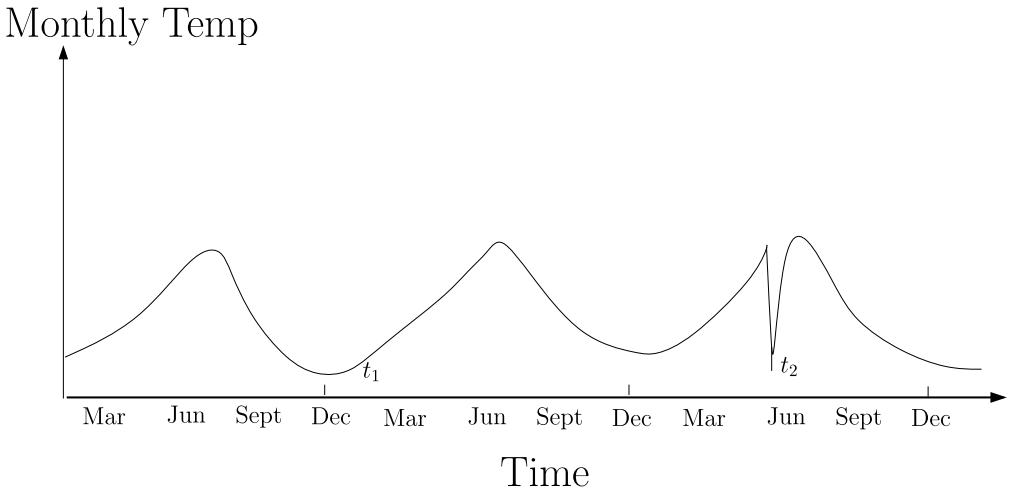
\includegraphics[width=0.7\textwidth]{contextual.png}
		\caption{Example of one contextual anomaly ($t_2$) in a monthly temperature time series dataset. Source: \cite{Kandhari2009}.}
		\label{fig:context_anom}
	\end{figure}
	
	\item \textit{Collective Anomaly}: When a group of data instances of a dataset may not be anomalies by themselves, but when they occur together they can be considered a collective anomaly.
	Figure \ref{fig:collective_anom} illustrates this type of anomaly using a human electrocardiogram output time series: the red values represent a collective anomaly, although that value by itself is not considered an anomaly (despite appearing several times during the dataset just by itself).
	
	\begin{figure}[!ht]
		\centering
		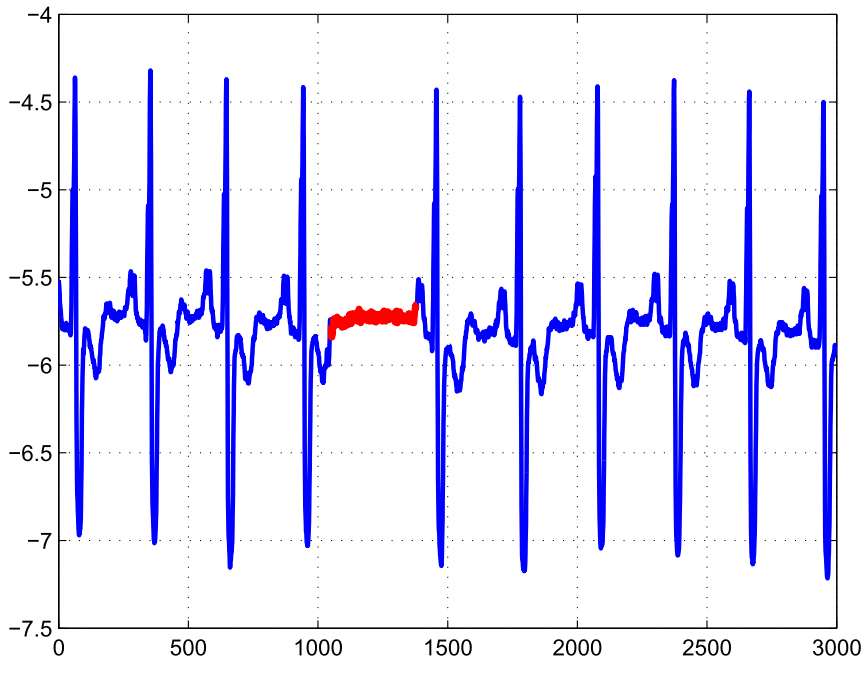
\includegraphics[width=0.6\textwidth]{collective.png}
		\caption{Example of one collective anomaly in a human electrocardiogram output time series dataset. Source:  \cite{Kandhari2009}.}
		\label{fig:collective_anom}
	\end{figure}
	
\end{itemize}

Because of the wide scope of each of these categories, this thesis will only focus on \textit{point anomalies} in the following sections and chapters. Information regarding the techniques capable of detecting contextual and collective anomalies can be found in Kandhari's survey on the topic (\cite{Kandhari2009}).

\section{Learning Mode} \label{sec:anomly_learn}

Anomaly Detection techniques can be classified based on the learning mode used:

\begin{itemize}
	\item \textit{Supervised}: Techniques using this learning mode assume that the data is fully labeled as either being \textit{normal} or \textit{anomalous}.
	Therefore, this constitutes a regular supervised learning classification problem. %However, it is important to note that in this case the classes are skewed (i.e. there will be have less anomalies in a dataset than \textit{normal} instances).
	
	\item \textit{Semi-supervised}: Techniques using this learning mode assume that the data only contains \textit{normal} examples and try to build a model that can learn the \textit{normal} behavior and identify examples that do not fit in this behavior.
	In the real-world this scenario is very frequent as in many domains it is difficult or expensive to measure anomalies and only \textit{normal} data is available.
	
	\item \textit{Unsupervised}: This learning mode does not require labeled data and assumes that the number of \textit{normal} instances is much higher than the number of \textit{anomalous} instances.
	Most of the Anomaly Detection techniques defined in the literature operate under this learning mode.
\end{itemize}


\section{Type of Techniques} \label{sec:anomaly_appr}

The techniques used in Anomaly Detection can be categorized into two groups according to their output \cite{Kandhari2009}:

\begin{itemize}
	\item \textit{Score output:} The techniques with this type of output assign a \textit{score} to each data instance that represents how much the instance can be considered an anomaly. The list of anomalous instances can then be retrieved by using manually defined thresholds on the scores or by marking all the top instances as \textit{anomalous}.
	
	\item \textit{Label output:} The techniques that output labels resemble regular binary-classifiers in Machine Learning by either classifying a data instance as being \textit{normal} or \textit{anomalous}. These techniques differentiate from the \textit{score} ones as they do not require any type of threshold definition after their application, as the data instance is already labeled as \textit{anomalous} or \textit{normal}.
\end{itemize}

\subsection{Classification Based Techniques}

Classification based techniques operate similarly to regular supervised learning classifiers: they train a model based on a set of labeled data and then classify each test data instance as being \textit{normal} or \textit{anomalous}.

One of the disadvantages of this group of techniques is that they require labeled data in the training phase of the model. Depending on the labels available in the training data, the techniques in this group can be subdivided into two types \cite{Kandhari2009}: multi-class and one-class.

%\textbf{TODO: Where does ``isolation forest'' algorithm fit?}

\subsubsection{Multi-class Techniques}\mbox{}

Multi-class techniques assume that the training data contains instances belonging to several different \textit{normal} classes and build a classifier that distinguishes each class from the remaining classes. These techniques classify a data instance as being \textit{anomalous} if they cannot classify it as one of the \textit{normal} classes \cite{Kandhari2009}.

Examples of these techniques include certain types of Neural Networks (e.g. Multi Layered Perceptrons, Hopfield Networks), Bayesian Networks, Rule Based techniques, Decision Trees and other binary and multi-class classifiers \cite{Kandhari2009}.

\subsubsection{One-class Techniques}\mbox{}

One-class techniques assume that the training data contains instances belonging to only one class -- the \textit{normal} one. The idea behind these techniques when learning the model is to define a decision boundary that isolates the \textit{normal} instances.
This decision boundary can therefore be used to classify new data: data instances that stay inside the decision boundry are are considered \textit{normal} and instances that stay outside the boundary are flagged as anomalies \cite{Kandhari2009}.
These techniques usually operate under the semi-supervised learning method presented in section \ref{sec:anomly_learn}.

Examples of these techniques include Replicator Neural Networks \cite{Hawkins}, Support Vector Machines (more specifically One-class SVMs \cite{Sc}) and Rule Based techniques \cite{Kandhari2009}).

\subsection{Nearest Neighbor Based Techniques}

Nearest Neighbor based techniques are based on the assumption that \textit{normal} data instances are situated in dense \textit{neighborhoods} of data instances, while \textit{anomalous} data instances situate themselves \textit{far} from other data instances.
The notion of \textit{neighboorhoods} and \textit{far} are employed with similarity/distance metrics that can evaluate how close (or far away) two data instances are.

These techniques can be subdivided into two different groups \cite{Kandhari2009}:
\begin{itemize}
	\item techniques that use the distance of each data instance to its $k^{th}$ nearest neighbor(s) as an anomaly score;
	
	\item techniques that use the concept of relative density of each data instance to compute an anomaly score (which will be detailed in this section).
\end{itemize}

\subsubsection{Density Techniques}\mbox{}

The assumption behind the density techniques is that a data instance that belongs to a neighborhood with low density (i.e. that contains only a few data instances) is \textit{anomalous}, while the opposite indicates that the instance is \textit{normal}.

\begin{figure}[!ht]
	\centering
	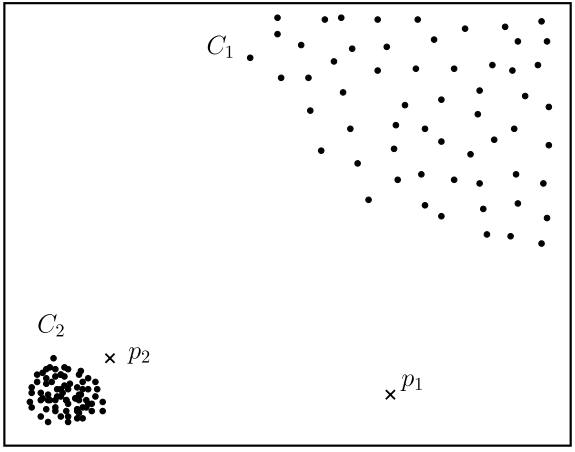
\includegraphics[width=0.6\textwidth]{density_anomalies.png}
	\caption{Example of a 2 dimensional dataset containing regions with different density values. Source: \cite{Kandhari2009}.}
	\label{fig:local_density}
\end{figure}

However, it is important to note that this assumption may not hold if the data has regions with different density values. Figure \ref{fig:local_density} illustrates this example with a 2 dimensional dataset: the distance of each of the instances in cluster $C_1$ to their nearest neighbor is higher than the distance of $p_2$ to its nearest neighbor in cluster $C_2$. Because of this the methods that are based on this assumption would not consider $p_2$ as an \textit{anomalous} instance although visually it is noticeable that this instance is \textit{anomalous} in the given feature space.

In order to overcome this limitation, some techniques within this category compare the density of the data instances to the density of their neighbors. One of the examples of this type of techniques is the LOF (Local Outlier Factor) \cite{Breunig}. Several techniques based on LOF	have been proposed more recently, either to adapt this algorithm to more complex data types or to improve its efficiency. Some examples include COF (Connectivity-based Outlier Factor) \cite{Tang2002}, ODIN (Outlier Detection using In-degree Number) \cite{Hautamaki2004} and LOCI (Local Correlation Integral) \cite{PapadimitriouS.KitagawaH.2003}.

\subsection{Clustering Based Techniques}

Clustering is a task in Data Mining in which the goal is to aggregate the data into meaningful or useful groups \cite{Tan2005}. Techniques that capture this idea have been applied to Anomaly Detection, out of which three groups of techniques can be distinguished in the literature based on their assumptions \cite{Kandhari2009}:

\begin{itemize}
	\item \textit{After clustering the data, \textit{normal} data instances belong to one of the clusters formed, while \textit{anomalous} data instances do not belong to any of the clusters}: several clustering algorithms (such as DBSCAN \cite{Ester:1996:DAD:3001460.3001507}) do not force all the data instances to belong to one of the clusters formed. With this particularity of the algorithms and under this assumption, we can consider these data instances as being \textit{anomalous}.
	
	\item \textit{\textit{Normal} data instances situate themselves close to their closest cluster's centroid, while \textit{anomalous} data instances remain far away from any cluster centroid}: these techniques usually use the distance of a data instance to its nearest cluster's centroid as an \textit{anomaly score}. Examples include the use of Self-Organizing Maps (SOM) \cite{Kohonen:1997:SM:261082}.
	It is important to note that if the \textit{anomalous} instances form a cluster by themselves, the techniques under this assumption will not be able to detect them.
	
	\item \textit{\textit{Normal} data instances situate themselves in large and/or dense clusters, while the \textit{anomalous} ones situate themselves in small and/or sparse clusters}: Examples of techniques that operate under this assumption include the FindCBLOF \cite{He:2003:DCL:770340.770389}.
\end{itemize}

\subsection{Statistical Techniques}

Statistical techniques operate under the assumption that \textit{normal} data instances occur in high probability regions of a statistical model, while \textit{anomalous} data instances occur in low probability regions \cite{Kandhari2009}.
These techniques consist in building a statistical model of the data, usually using \textit{normal} data instances, similarly to the One-class Classification techniques. However, it is important to note that these techniques have a different assumption from One-class techniques: Statistical techniques are based on statistical models and data instances are considered anomalous if they have a low probability of being generated from the learned model. One-class Classification techniques, however, are based on classification models and in the definition of a decision boundary between instances. In this case, the decision of whether a data instance is \textit{anomalous} or not relies only in the location of the instance within the decision boundary.

The literature distinguishes parametric and non-parametric techniques, which will be detailed in this section.

\subsubsection{Parametric Techniques}\mbox{}

Parametric techniques are characterized by making assumptions on the distribution of the data (e.g. assuming it follows a Gaussian distribution or it can be modeled linearly) and build a statistical model of the data, by learning its parameters with \textit{normal} data instances.
The anomaly score of a new data instance can then be calculated from the probability density function of the learned model (if the instance locates itself in a region where the function has a low value it may be considered \textit{anomalous} and vice-versa).
Along with this approach, some techniques also use statistical hypothesis testing to assess if a new data instance is \textit{anomalous} or not.

These parametric techniques can be subdivided into different groups:

\begin{itemize}
	\item \textit{Gaussian Model}: techniques that assume the data distribution is Gaussian. These techniques detect \textit{anomalous} data instances based mostly on thresholds. One simple example of this type of techniques is the box plot rule  \cite{laurikkala2000informal}.
	\item \textit{Regression Model}: techniques that fit a linear model to the data. These techniques consider that a data instance is anomalous if its residual value is above a threshold. Linear models such as robust regression \cite{leroy1987robust} have been used in these techniques.
	\item \textit{Mixture of Parametric Distributions}: techniques that either model \textit{normal} and \textit{anomalous} data instances as belonging to two different distributions, or by modeling the \textit{normal} data instances as belonging to a mixture of data distributions.
\end{itemize}

\subsubsection{Non-parametric Techniques}\mbox{}

Unlike the parametric techniques, the non-parametric approaches do not make any assumptions about the statistical distributions of the data.

These techniques, as well as the parametric ones, can be subdivided into different groups:

\begin{itemize}
	\item \textit{Histogram Based}: these techniques use histograms to maintain a profile of the data (usually only containing \textit{normal} instances). The \textit{anomaly score} of a new data instance is high if it falls in a bin of the histogram with low frequency, and vice-versa.
	\item \textit{Kernel Function Based}: these techniques use kernel functions to estimate the probability distribution function, by using \textit{normal} data instances. The \textit{anomaly score} of a new data instance is high if it falls in a area with low probability, and vice versa.
\end{itemize}

\subsection{Information Theoretic Techniques}

Information theoretic techniques analyze the information content of the data with information theory measures (e.g. Kolomogorov Complexity, Entropy) and are based on the assumption that \textit{anomalous} data instances induce irregularities in the information content of the data \cite{Kandhari2009}.

\subsection{Spectral Techniques}

Spectral techniques are based on the assumption that \textit{normal} and \textit{anomalous} data instances can be distinguished in a lower feature subspace (i.e. in a new dataset with a lower number of features). These techniques often use Principal Component Analysis (PCA) \cite{Jolliffe2002} to project the data into a lower feature space.

%\section{Benchmarking}

%\subsection{Previous Works}

%\subsection{Evaluation Metrics}

%\subsection{Datasets for Evaluation - Delete this!} 
\chapter{Ensemble Learning and Stacked Generalization} \label{chap:ensemble}

\section*{}

This chapter provides an overview over the concepts of Ensemble Learning and Stacked Generalization.

The field of \textit{Ensemble Learning} is presented briefly, with examples of general as well as more specific approaches used in the field of Anomaly Detection. 
Finally, the concept of \textit{Stacked Generalization} is presented as well as several approaches that are used in this field.

\section{Ensemble Learning Definition}\label{sec:ensemble_def}

Based on the definition provided by \textcite{Mendes-Moreira2012}, Ensemble Learning can be defined as:

\begin{definition}[Ensemble Learning] \label{def:ensemble_learning}
	Ensemble Learning is a process that uses a set of models (ensemble), each of them obtained by applying a learning algorithm to a given problem. This set of models is integrated in some way to obtain the final output.
\end{definition}

It is important to note that this definition is independent of the learning mode, which means that Ensemble Learning can be used for supervised and unsupervised learning \cite{Mendes-Moreira2012}.
Although Ensemble Learning is more frequently applied in supervised learning (classification and regression), it has also been used in clustering \cite{Strehl:2003:CEK:944919.944935}.

However, given the wide scope of these applications, this chapter and the following ones will only focus on classification applications of Ensemble Learning.

Formally, a classification model (or hypothesis) $m = (L, P, \mathcal{D})$ is an application of a learning algorithm $L$, with a set of defined parameters $P$ and trained on a dataset $\mathcal{D} = \{(x_i, y_i), i = 1, \dots, N\ \}$, where $x_n$ represents the feature values of the $n^{th}$ instance and $y_n$ the class value of the $n^{th}$ instance.
%\textbf{COMPLETAR} Each instance $x_i$ has $M$ features
Given a data instance $x_i$ from a dataset $\mathcal{D}$, $m(x_i)$ is the prediction of the class value of $x_i$ made by model $m$.

Therefore, an ensemble $E = \{m_j, j = 1, \dots, J \}$ can be defined as a set of $J$ models, where $E(x_i) = g(m_1, \dots, m_J)$ corresponds to the prediction of the class value of $x_i$ by the ensemble $E$. This prediction is made using an aggregation function $g$ which combines the predictions from the $J$ models of the ensemble, $m_1(x_i), m_2(x_i), \ldots, m_J(x_i)$.
It is important to mention that this definition is recursive, as an ensemble can also be considered a model in another ensemble.
The different ways in which the set of models can obtained and then integrated to obtain a final output will be discussed further in this section.

%It is important to mention that this definition is recursive, as an ensemble can also be considered a model in another ensemble.

It is also important to refer that approaches with \textit{Multiple Models} or \textit{Multiple Learners} presented sometimes throughout the literature refer to the same concept presented in this section \cite{Mendes-Moreira2012}.

\textcite{Dietterich1990} presents three reasons why Ensemble Learning can lead to better results:

\begin{itemize}
	\item Applying a learning algorithm to a specific problem can be interpreted as searching for the best model for this problem (the one that is considered the \textit{best} according to a predefined metric) within a space of possible models $\mathcal{H}$. When the dataset provided is too small compared to the space $\mathcal{H}$, several models can be equally considered the \textit{best}. By building an ensemble of this set of models, it is possible to obtain a new model that may generalize better to new data.
	
	\item Some learning algorithms generate models for a specific problem by performing an optimization process over an error function, which can get stuck at a local minimum. This is the case, for example, of neural network algorithms. By building an ensemble of different models (obtained by starting this optimization at a different starting points), it is possible to obtain a model that is closer to the global minimum.
	
	\item Given a specific problem, a learning algorithm works by instantiating a model the mimics the underlying process that can explain this problem (we will represent this process by $f$). However, some learning algorithms (e.g. linear algorithms) may not have a model space $\mathcal{H}$ large enough to contain a model that can represent $f$ accurately. By building an ensemble of different models and combining their outputs, it may be possible to expand the model space $\mathcal{H}$ and have a better approximation of $f$.
\end{itemize}

\textcite{hansen1990neural} however state that there are two necessary (and sufficient) conditions for an ensemble of models to be more accurate than any of individual models that belong to it:

\begin{itemize}
	\item Each of the models that compose the ensemble must be \textit{accurate}, which according to the author is to be better than random guessing.
	
	\item The ensemble of models should be \textit{diverse} (i.e. the outputs of the models should be uncorrelated to each other).
\end{itemize}

\section{Ensemble Learning Process}

\textcite{Mendes-Moreira2012} proposes three phases to be considered when using Ensemble Learning (illustrated in figure~\ref{fig:ensemble_process}), which will be detailed in this section. 

\begin{figure}[ht!]
	\centering
	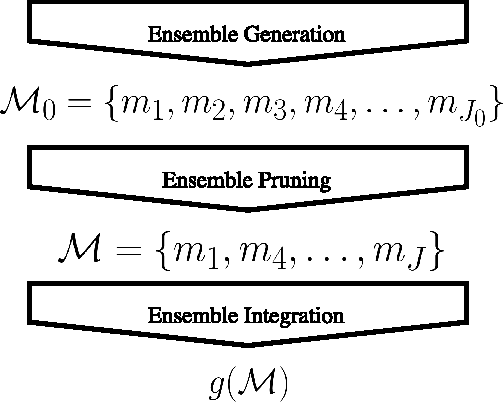
\includegraphics[width=0.5\textwidth]{figures/Ensemble_Process.pdf}
	\caption{Scheme representing the Ensemble Process. Adapted from \cite{Mendes-Moreira2012}.}
	\label{fig:ensemble_process}
\end{figure}

\subsection{Ensemble Generation}\label{sec:ens_gen}

The initial step in the process of Ensemble Learning is to generate an ensemble of models. We are interested in generating a set of models $\mathcal{M}_0 = \{ m_j, j = 1, \dots, J_0 \}$.

Ensembles can be of two different types \cite{Mendes-Moreira2012}:

\begin{itemize}
	\item \textit{Homogeneous}: when the set of models are generated by the same learning algorithm (e.g. tuned with different parameter settings). Most of the research work in Ensemble Learning is conducted with this type of ensembles \cite{Mendes-Moreira2012}.
	\item \textit{Heterogeneous}: when the set of models are generated by different learning algorithms. This type of ensembles may have more diversity between models than the homogeneous type, if the nature of the learning algorithms is diverse enough \cite{Mendes-Moreira2012}.
\end{itemize}

It is interesting to note that homogeneous ensembles can be used in heterogeneous ensembles, given the recursive definition of an ensemble.

A possible methodology that can be followed is the \textit{overproduce-and-choose} approach.
In this methodology a high number of models are generated in the ensemble generation phase (``overproduce''), leaving the task of selecting the best models to the pruning phase (``choose'').	

\textcite{Mendes-Moreira2012} presents different ways to produce different models in both homogeneous and heterogeneous ensembles, which will be detailed in this section.

\subsubsection{Data Manipulation Approaches}\label{sec:data_manipulation}

In the definition of a model $m = (L, P, \mathcal{D})$, these approaches perform changes in the dataset $\mathcal{D}$ used to train the learning algorithm $L$. The same learning algorithm is trained with different datasets will result in different models (which may or may not be diverse among themselves, depending on the sensitivity of the algorithm and its sensibility to the training dataset).

\paragraph{Subsampling from the Training Set}\mbox{}

This type of approach generates different models using different subsamples of the same dataset.
One of the most popular approaches is $bagging$ (bootstrap aggregating), which generates $k$ subsamples of a dataset $\mathcal{D}$.
These subsamples are made with replacement (a subsample can contain a data instance more than once).
A model is then trained with each of the $k$ subsamples generated, generating $k$ different models.

\paragraph{Manipulating the Input Features}\mbox{}

This type of approach can be divided in two subtypes:

\begin{itemize}
	\item \textit{Feature Selection}: 
	A feature selection process is performed on the dataset, in order to generate different datasets (each one with a different subset of features).
	One example of this approach is the \textit{random subspace} method \cite{ho1998random} (which chooses randomly feature subsets randomly).
	
	\item \textit{Feature Transformation}:
	A transformation is conducted on the features' original values, in order to generate different datasets with different features.
	One example is the \textit{input smearing} approach \cite{Frank2006} that adds gaussian \textit{noise} to each numeric feature.
\end{itemize}

\textit{Rotation forests} (proposed by \textcite{1677518}) incorporates both feature selection and transformation processes. First, this method selects different $k$ disjoint subsamples of features. Then, for every subsample, PCA is performed to project the feature space into a new one, where the new features correspond to linear combinations of the original ones.

\subsubsection{Model Generation Manipulation}

This type of approaches manipulates the learning algorithm's parameters or learning conditions.

\paragraph{Manipulating the Parameter Set}\mbox{}

Manipulating the parameter set of a learning algorithm is a possibility to generate different models, either by iterating by ranges of possible values (Grid Search \cite{hsu2003practical}) or using a Random Search \cite{bergstra2012random}.

\paragraph{Manipulating the Induction Process}\mbox{}

In order to to obtain a model $m$ from a learning algorithm $L$ on a dataset $\mathcal{D}$ it is necessary to perform \textit{induction}. This type of approaches try to change the way in which the model is generated, allowing the generation of models under different induction conditions.
One of the most common approaches is to change the error function in optimization-based learning algorithms (such as neural networks).

\paragraph{Manipulating the Generated Model}\mbox{}

This type of approaches performs adjustments on an already generated model, leading to different models.
One known approach is to change a Classification Association Rules (CARs) model by subsampling the model's set of rules $n$ times, generating $n$ models with different sets of rules. 

\subsection{Ensemble Pruning}

The generation of an ensemble in the previous phase, although might guarantee a wide diversity of models, it does not guarantee that the smallest ensemble possible with maximum accuracy was obtained. Several of the models may also have very correlated outputs, which do not add any extra knowledge to the final prediction.
Also, since some of the approaches for generating ensembles involve randomness, there is no guarantee all the models in the ensemble will contribute positively to the final prediction.

Therefore the goal of Ensemble Pruning is to improve the predictive accuracy of the ensemble and reduce the \textit{cost} of the ensemble (since an ensemble with a higher number of models will be more computationally costly to use).

Ensemble Pruning consists in selecting a subset $\mathcal{M}$ with $J$ models of the set of models generated in the previous step.
This phase corresponds to the ``choose'' step of the \textit{overproduce-and-choose} methodology presented in section \ref{sec:ens_gen}. Therefore:

\begin{equation}
\mathcal{M} \subseteq \mathcal{M}_0
\end{equation}

% DESCOMENTAR
%A possible heuristic to choose the models can be, for example, based on a combination of diversity and/or accuracy of the models. Several metrics suitable for measuring diversity and accuracy will be discussed further in this chapter, in section \textbf{PREENCHER COM A SECTION}.

\textcite{Mendes-Moreira2012} proposes two types of approaches for conducting Ensemble Pruning, which will be detailed in this section.

\subsubsection{Partition-Based Approaches}

The main idea of partition-based approaches is to cluster the models into several groups. This could be done, for example, with the clustering algorithm k-means, in order to obtain a set of clusters of similar models.
Afterwards, one or more representative models from each group are chosen to constitute the pruned ensemble.

\subsubsection{Search-Based Approaches}

Search-based approaches can divided in three different types:

\begin{itemize}
	\item \textit{Exponential Search Approaches}: Exponential Search Approaches search the complete search space of possible models to be included from $\mathcal{M}_0$. This search space has $2^{J_0} - 1$ possible subsets of models and the search for the optimal subset is an NP-complete problem.
	
	\item \textit{Randomized Search Approaches}: Randomized Search Approaches perform a heuristic search in the search space (e.g. using evolutionary algorithms). Approaches such as genetic algorithms, tabu search and population-based incremental learning have been used in previous works \cite{Ruta2001}.
	
	\item \textit{Sequential Search Approaches}: Sequential Search Approaches perform a search by iteratively adding and/or removing a model from subset to maximize some criteria.
	This can be done using using \textit{Forward Subset Selection}, \textit{Backward Subset Selection} or a combination of both.
	In \textit{Forward Subset Selection}, the search starts with am empty ensemble and models are iteratively added.
	In the case of \textit{Backward Subset Selection}, the search starts with all the possible models generated in the ensemble and they are iteratively removed.
\end{itemize}

\subsection{Ensemble Integration}\label{sec:ensemble_integration}

The final step in Ensemble Learning is the combination of the predictions from the models in the ensemble.

In classification, the most popular approaches to combine models can be divided into two categories: combination-based approaches and model-based approaches.

\subsubsection{Combination-based Approaches}

Combination-based approaches are based on combination rules of the class values outputted by the models in the ensemble.
First it is important to define the decision of the $j^{th}$ model (referred in section \ref{sec:ensemble_def} as \textit{class value}) as $d_{j,c} \in \{ 0,1 \}, j = 1, \dots, J$ and $c = 1, \dots, C$, where $J$ is the number of models in the ensemble (as defined previously in section \ref{sec:ensemble_def}) and $C$ is the number of classes.
If the $j^{th}$ model outputs class $c$, then $d_{j,c} = 1$ and 0 otherwise.

\paragraph{Majority Voting}\mbox{}

Majority Voting has three different subtypes, in which the ensemble output corresponds to the class predicted by all classifiers (\textit{unanimous voting}), the class predicted by at least one more than half the number of classifiers (\textit{simple majority}) or the class predicted by the majority  of the classifiers, even if it is predicted by less than half of the number of classifiers (\textit{plurality voting}) \cite{Polikar2012a}.

The Majority Voting approach (unless specified otherwise) usual refers to \textit{plurality voting} \cite{Polikar2012a} and the decision of which class value to output can be defined as follows: 

\begin{equation}\label{eq:majority}
\text{arg}\max_c \sum_{j = 1}^{J} d_{j,c}
\end{equation}

\paragraph{Weighted Majority Voting}\mbox{}

If it is known that some of the models are more likely to make correct predictions than others, weighting the decisions of the models can improve the performance of the Majority Voting approach \cite{Polikar2012a}.
In this case, models with higher performance would have a bigger weight assigned and models with a worse performance otherwise.
We define the weight of a model $m_j$ as $w_j$.
These weights usually are normalized so that:

\begin{equation}
w_j \in [0, 1] \ \wedge \ \sum_{c = 1}^{C} w_{j} = 1, \ j = 1, \dots, J
\end{equation}

In this case, the decision of the class output is defined as follows:

\begin{equation}
\text{arg}\max_c \sum_{j = 1}^{J} w_j \cdot d_{j,c}
\end{equation}

A estimation of the weights could be performed by estimating the models' generalization performance in a separate validation set.

\paragraph{Borda Count}\mbox{}

The Board Count method assumes that each model is capable of ranking its support to each class $c$ and takes this into consideration \cite{Polikar2012a}. This method can be particularly useful in multi-class problems where $C$ takes a considerable value.

For each model $m_j$, each class $c$ receives $C-r$ votes being $r$ the position of $c$ in the ranking belonging to model $m_i$.
For example, if $C = 4$ and the class 1 is ranked $3^{rd}$ by model $m_1$ (meaning that model $m_1$ picked class 1 as being the third most probable), then class 1 will receive $4-3 = 1$ votes.
This procedure is then executed for each model and possible class value, the results are added up and the class with higher number of votes is chosen.

\subsubsection{Model-based Approaches}

Throughout the literature in Ensemble Learning, several more complex methods of prediction combinations are described \cite{Polikar2012a}.
Some of these can be considered model-based, in the sense that there is a training phase of an algorithm that ``learns'' how to combine the several models in the ensemble.
We will describe briefly two possible approaches in this section.

\paragraph{Stacked Generalization}\mbox{}

\begin{figure}[ht!]
	\centering
	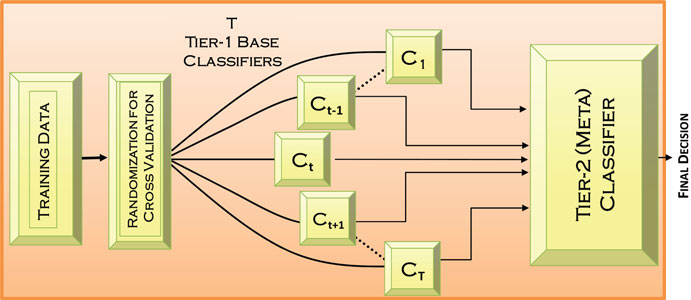
\includegraphics[width=0.8\textwidth]{figures/stacking}
	\caption{Scheme of the Stacked Generalization approach. Source: \cite{Polikar2012a}.}
	\label{fig:stacking}
\end{figure}

Stacked Generalization (also known as Stacking) is an Ensemble Learning method in which the predictions of the models are combined using another model (also known as a \textit{meta-classifier}) \cite{Polikar2012a}. In order to do so, a new dataset is generated using the prediction outputs of the models belonging to the ensemble.
This new dataset is then used to generate another model (the \textit{meta-classifier}).
This mechanism is illustrated in figure \ref{fig:stacking}.

This approach can be seen as an extension of the Weighted Majority Voting.
However, unlike this method, the impact of each model in the final decision is not translated into a single value.
Stacking determines which models are likely to be accurate in different parts of a dataset's feature space, since certain models may be more ``specialized'' in predicting correctly certain data instances.
In this case the predictions of these models for these data instances will have a higher ``weight'' and the remaining models a lower one.

Since this approach is the main focus of this dissertation, we will focus on it later in this chapter.

\paragraph{Mixture of Experts}\mbox{}

\begin{figure}[ht!]
	\centering
	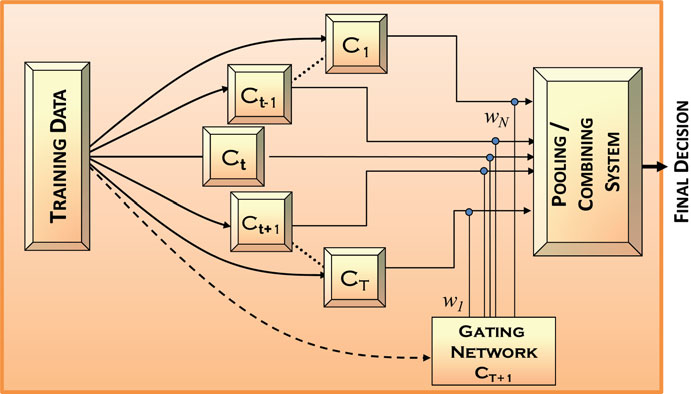
\includegraphics[width=0.8\textwidth]{figures/mixture_models}
	\caption{Scheme of the Mixture of Experts approach. Source: \cite{Polikar2012a}.}
	\label{fig:mixture}
\end{figure}

As the name reflects, the Mixture of Experts approach assumes certain individual models may be \textit{experts} in predicting the class value for certain data instances but more inaccurate for the remaining ones in the dataset. This background idea is very similar to the one behind Stacking, in which weights are assigned to each model of the ensemble reflecting its accuracy in certain parts of the dataset's feature set.

However, these weights are not determined by a new model but by a \textit{gating network} (as illustrated in \ref{fig:mixture}).
This gating network is trained using the expectation-maximization (EM) algorithm on the original dataset.

\section{Ensemble Learning Applications to Anomaly Detection}

Ensemble Learning has been previously used with Anomaly Detection techniques \cite{Aggarwal:2013:OA:2436823}.
Because these applications were typically based on unsupervised learning, we will focus on these in this section.
Several applications using Stacking (and therefore supervised learning based) will be discussed in the next section.
%We distinguish two types of approaches, based on the learning mode of the Anomaly Detection techniques: supervised learning approaches and unsupervised learning approaches.


%\subsection{Supervised Learning Approaches}

\subsection{Unsupervised Learning Approaches}

%The majority of applications of Ensemble Learning to Anomaly Detection are associated with unsupervised learning approaches.
\textcite{Aggarwal:2013:OA:2436823} classifies unsupervised learning approaches as being either sequential or independent.

\subsubsection{Sequential Approaches}

In sequential approaches, several models are applied sequentially either to the entire dataset or portions of it \cite{Aggarwal:2013:OA:2436823}.
The underlying assumption of this group of approaches is that the application of each algorithm allows a more refined execution by either modifying the data or the subsequent models.
Data modifications could include some of the approaches described in section~\ref{sec:data_manipulation}, such as subsampling the dataset, performing feature selection and feature transformation \cite{Aggarwal:2013:OA:2436823}.
The final decision can be either the decision of the last applied model or a combination of the several models applied.

Models in earlier stages of a sequential approach could, for example, remove more obvious \textit{anomalous} instances of the data so that latter models perform a more robust anomaly detection {\cite{Aggarwal:2013:OA:2436823}.
The latter might then be able to have a better understanding of less-noticeable \textit{anomalous} instances the data.
This can be used, for example, with clustering based techniques, in which more robust clusters can be built after the most \textit{anomalous} instances are removed \cite{Barbara:2003:BDM:952532.952616}.

\subsubsection{Independent Approaches}

In independent approaches, several models are used without having any effect on one another.
These models can be applied either to the entire dataset or to portions of it \cite{Aggarwal:2013:OA:2436823}.
The underlying assumption of these approaches is that several Anomaly Detection techniques can be specialized on certain instances of the dataset, so therefore an application of these techniques and consequent combination of predictions might lead to more accurate decision.
The methodologies to generate the models in these approaches include some of the ones already described in section~\ref{sec:ens_gen}, such as feature selection and dataset subsampling.

Some approaches within this category use models with the LOF (\cite{Breunig:2000:LID:335191.335388}) and LOCI (\cite{PapadimitriouS.KitagawaH.2003}) learning algorithms.	

\subsubsection{Ensemble Integration}

One of the difficulties with unsupervised learning Anomaly Detection techniques is that they usually output a numeric score.
Different techniques can output scores in different scales as, some techniques might output a normalized score (e.g. LOF), where others might output a raw distance score (e.g. k-nearest neighbor) \cite{Aggarwal:2013:OA:2436823}.
Different techniques might also have a different ordering of the scores, as some techniques output larger scores for \textit{anomalous} instances, while others output smaller scores for this type of instances \cite{Aggarwal:2013:OA:2436823}.
Therefore, it is important to normalize the scores of each technique so that they can be meaningfully combined without over-weighting specific techniques \cite{Aggarwal:2013:OA:2436823}.

\paragraph{Normalization of Scores}\mbox{}

The first step is to make sure that each model of the ensemble has the same ordering of the scores.
This can be solved by flipping the sign of the scores of the models in which lower score values correspond to higher probability of being an anomalous data instance.
By doing this, in every technique a higher score will always correspond to a higher probability of a data instance being anomalous.

The second step is to convert the scores of the different models into comparable values.
\textcite{Aggarwal:2013:OA:2436823} presents two possible methods:

\begin{itemize}
	\item \textit{Range-based scaling}:
	Range-based scale uses the maximum and minimum scores of one model for a specific dataset to convert the scores.
	The converted scores will then lie in the interval $[0,1]$.
	
	Let $s_j(x_i)$ the score that the model $m_j$ outputs for a data instance $x_i$ and let $max_{j}$ and $min_{j}$ be the maximum and minimum value respectively of the scores of model $m_j$ for a dataset $\mathcal{D}$.
	The converted score of a data instance $x_i$ with a model $m_j$ takes the following value $s'(x_i)$: 
	
	\begin{equation}
	s_j'(x_i) = \frac{s_j(x_i) - min_j}
	{max_j - min_j}
	\end{equation}
	
	The disadvantage of this method is that the values of the converted scores will depend highly on the values of $max_j$ and $min_j$.
	For example, in most Anomaly Detection techniques the value of $max_j$ is attributed to the most \textit{anomalous} data instance.
	In some datasets this score might be much larger than the scores of the other data instances.
	This phenomena can reduce drastically the discrimination of the remaining scores and reduce the ability of distinguishing which ones might be \textit{anomalous} \cite{Aggarwal:2013:OA:2436823}.
	
	\item \textit{Standardization}: 
	Standardization converts the scores into standard scores (also known as Z-values).
	
	Let $\mu_j$ and $\sigma_j$ be the mean value and standard deviation respectively of the scores of model $m_j$ for a dataset $\mathcal{D}$.	
	The converted score of a data instance $x_i$ with a model $m_j$ takes the following value $s_j'(x_i)$:
	
	\begin{equation}\label{eq:standardization}
	s_j'(x_i) = \frac{s_j(x_i) - \mu_j}{\sigma_j}
	\end{equation}
	
	This method however, assumes that the scores of each model $m_i$ follow a gaussian distribution. Although this assumption rarely holds, it is reported that this method usually provides reasonably robust results \cite{Aggarwal:2013:OA:2436823}.
	
\end{itemize}

Another method, discussed by \textcite{Gao:2006:COS:1193207.1193286}, is to convert the techniques' scores into probabilities using the EM algorithm.

\paragraph{Combination of Scores}\mbox{}

After the scores of the different techniques are normalized they can be combined.
Note that the approaches discussed in section~\ref{sec:ensemble_integration} can not be used, since the score is a real number and not a nominal number.

\textcite{Aggarwal:2013:OA:2436823} presents two possible combination methods:

\begin{itemize}
	\item \textit{Averaging}:
	The final score is computed as the mean of the scores of the different models. Therefore, a data instance $x_i$ will have the following score:
	
	\begin{equation}
	\frac{\sum_{j = 1}^J s_j(x_i)}{J} 
	\end{equation}
	
	\item \textit{Maximum}:
	The final score is computed as the maximum score across the different models. Therefore, a data instance $x_i$ will have the following score:
	
	\begin{equation}
	\max_{j} \ s_j(x_i) \ , \ j = 1, \dots, J 
	\end{equation}
	
\end{itemize}

\section{Stacked Generalization}\label{sec:stacking}

Stacked Generalization (also known as Stacking) was proposed initially by \textcite{wolpert1992stacked}.
It consists of an ensemble method with three steps: 1) models are generated using one or more learning processes; 2) a new dataset is generated with the predictions of those models, together with the original target variable; and 3) a new model is obtained using the new dataset containing the predictions of the previous models~\cite{Sesmero2015}.
We refer to the models in the ensemble as the \textit{level-0 models}, their outputs as \textit{metafeatures} and the model built with them as the \textit{level-1 model} or \textit{meta-classifier}.

%\textbf{MUDAR J e F PARA OUTRA LETRA}
Formally, given a dataset $\mathcal{D}^0$, Stacking first generates a set of mutually exclusive partitions of approximate size $\mathcal{D}^0_1, \dots, \mathcal{D}^0_Z$. Then, similarly to a \textit{Z}-fold cross-validation procedure, at each iteration $z$, the method omits the subset $D^0_z$ and uses the subset $D^0 - D^0_z$ as a training set to generate $M$ level-0 models by training several learning algorithms.%
After the level-0 models have been generated for each
iteration $z$, they are applied to the dataset $D_z$ to obtain the predictions that will be used as the level-1 dataset values. We will refer to this dataset as the meta-dataset $\mathcal{D}^1_z$. The process is repeated for all $Z$ datasets and the complete level-1 dataset, $D^1$ is defined as:

\begin{equation}
\bigcup\limits_{z=1}^{Z} \mathcal{D}^0_z
\end{equation}

The dataset $\mathcal{D}^1$ has the same number of rows as $\mathcal{D}^0$, but $M$ features (whose values are the predictions of the $M$ level-0 models) plus the class value.
The dataset $\mathcal{D}^1$ can then be used to train a learning algorithm, which becomes the level-1 model~\cite{Sesmero2015}.

To classify a new instance $x_i$, the level-0 models produce a vector of predictions ${m_1(x_i), \dots, m_M(x_i)}$.
This vector is the input to the level-1 model, which makes a prediction regarding the class value of $x_i$.

\subsection{Applications to Anomaly Detection}

The application of Stacking for Anomaly Detection is recent and sometimes not very transparent and easy to track.
However, we can emphasize two approaches in the literature:

\begin{itemize}
	\item \textcite{Micenkova} presented a Stacking Generalization methodology for Anomaly Detection, using outputs from two unsupervised Anomaly Detection techniques (k-NN outlier and LOF).
	Among with these two techniques, the authors used feature bagging which consists in a feature selection approach to generate different models from the same learning algorithms.
	The meta-classifier used in this approach was a model based on the Logistic Regression learning algorithm with L1 Regularization.
	
	\item \textcite{Cerqueira2016} proposed an approach similar to Stacking, in which the predictions from several models (LOF and Hierarchical Agglomerative Clustering) were added to the original dataset. According to our notation, the dataset used in this work has the features from $\mathcal{D}^0$ and $\mathcal{D}^1$.
	The meta-classifier used in this approach was a model based on the XGBoost learning algorithm.
\end{itemize}

%lala

\chapter{Experimental Methodology} \label{chap:meth}

\section*{}

In order to study the application of Stacking to the problem of Anomaly Detection, first several techniques were evaluated concerning their predictive performance as well as the diversity among themselves, since these are the two concepts that need to be present in order to obtain better performances using Ensemble Learning methods (as described in section~\ref{sec:ensemble_def}).
Afterwards, a study using the same techniques was conducted using Stacking approaches and their performance was analyzed.

This chapter will describe the experimental methodology followed throughout this thesis, more specifically:

\begin{itemize}
	\item The first experimental study, focused on the performance and diversity of several Anomaly Detection techniques.
	\item The second experimental study on the performance of Stacking approaches using some of the Anomaly Detection techniques used on the first study.
\end{itemize}

\section{Objectives}

The original idea of this experimental research was to measure the performance and diversity of each of the techniques available and, based on these results, select the best techniques to group in an ensemble and evaluate its performance.

Given a dataset $\mathcal{D}$ divided in three mutually exclusive partitions of approximate size $\mathcal{D}_1$, $\mathcal{D}_2$, $\mathcal{D}_3$, we could separate this experimental research into three phases (as illustrated in figure~\ref{fig:ensemble_process}):

\begin{enumerate}
	\item \textit{Ensemble Generation}: Select a diverse group of Anomaly Detection techniques to obtain models from.
	
	\item \textit{Ensemble Pruning}: Evaluate these potential models on the partition $\mathcal{D}_1$ using a cross-validation methodology (successively train a model on a set of partitions and test on a different partition) and select the top models with better performance to integrate in a ensemble $\mathcal{M}$.
	
	\item \textit{Ensemble Integration}: Select several possible Stacking approaches (i.e. usings a few models from $\mathcal{M}$, different meta-classifiers, \dots) and evaluate each of these approaches on the partition $\mathcal{D}_2$ using a cross-validation methodology.
	After this evaluation is performed, the best Anomaly Detection algorithm on $\mathcal{D}_1$ and the best Stacking approach on $\mathcal{D}_2$ would then be evaluated on partition $\mathcal{D}_3$ in order to conclude if the use of Stacking could lead to a better performance.
\end{enumerate}

However, given the fact that the datasets used for evaluation of this thesis do not have a large number of instances (see section~\ref{sec:datasets}), this division would reduce the number of instances for each of the partitions $\mathcal{D}_1$, $\mathcal{D}_2$, $\mathcal{D}_3$.

Thus, the main premises of this work is that among the models we have available there are some that are accurate and some that are diverse.
This is however a relaxation from the conditions described in section~\ref{sec:ensemble_def}.
Therefore, the methodology followed was:

\begin{enumerate}
	\item \textit{Experimental study on Anomaly Detection techniques}: Choose a set of Anomaly Detection techniques and examine their performance and diversity using the entire dataset $\mathcal{D}$.
	The goal of this study would be to evaluate if we are in the presence of at least some accurate and/or diverse models.
	
	\item \textit{Experimental study on Stacking approaches}: Choose a set of Stacking approaches (using different level-0 models and different level-1 models) and evaluate their performance on $\mathcal{D}$. Finally, conclude if the Stacking approaches perform better than the individual model performances.
\end{enumerate}

\section{Study on Anomaly Detection Techniques}

This first study conducted during this experimental research had the following objectives:

\begin{itemize}
	\item Study the performance and diversity of different types of Anomaly Detection techniques on several well-known datasets;
	
	\item Assess if this experimental setup contains accurate and diverse models.
\end{itemize}

\subsection{Anomaly Detection Techniques}\label{sec:study_techniques}

Techniques from several of the groups presented in chapter~\ref{chap:anomaly} were used in this study, more specifically Classification based techniques, Nearest Neighbor based and Clustering based. These algorithms are listed in table~\ref{tab:nanomaly} and will be specified in this section according to their learning mode (i.e. supervised, semi-supervised and unsupervised).
Statistical, Information Theoretic, and Spectral based techniques were not used in this study due the lack of implementations of techniques in these groups for multivariate data.
A technique that predicts randomly if a data instance is \textit{anomalous} or not was used in order to define the baseline of performance in each dataset. 

\begin{table}[!ht]
	\centering
	\caption{Anomaly Detection techniques used in this study for each nomenclature group and learning mode.}
	\label{tab:nanomaly}
	\begin{tabular}{@{}lp{3cm}p{3cm}p{2.5cm}@{}}
		\toprule
		& \textbf{Supervised} & \textbf{Semi-Sup.} & \textbf{Unsupervised} \\ \midrule
		Classification & CART, SVM, NB, RF, MLP & One-class SVM & - \\
		Nearest Neighbors & - & - & LOF \\
		Clustering & - & - & DBSCAN, \newline k-means \\
		Statistical & - & - & - \\
		Information Theoretic & - & - & - \\
		Spectral & - & - & - \\ \bottomrule
	\end{tabular}
\end{table}

It is also important to point out that these techniques can have different types of outputs:

\begin{itemize}
	\item \textit{Binary}: A binary value indicating if a data instance is \textit{anomalous} or not.
	\item \textit{Probabilistic}: A numeric value that is always contained in the interval $[0,1]$ and can be interpreted as the probability of a data instance being \textit{anomalous}.
	\item \textit{Other Numerical}: A numerical value that is not in the interval $[0,1]$ and does not represent a probability.
\end{itemize}

The classification of the techniques according to its output is presented in table~\ref{tab:anoutput}.

\begin{table}[!ht]
	\centering
	\caption{Anomaly Detection techniques used in this study regarding the type of output.}
	\label{tab:anoutput}
	\begin{tabular}{@{}l|l|l@{}}
		\toprule
		\textbf{Binary} & \textbf{Probabilistic} & \textbf{Other Numerical} \\ \midrule
		One-class SVM & CART, SVM, NB, RF, MLP & k-means, DBSCAN, LOF \\ \bottomrule
	\end{tabular}
\end{table}

%\textbf{Três tipos de outputs dos algoritmos:}
%- Binário
%- Probabilístico
%- Score de ranking

%Livro do aggarwal: If the threshold is selected too restrictively to minimize the number of declared outliers, then the algorithm will miss true outlier points (false negatives). On the other hand, if the algorithm declares too many data points as outliers, then it will lead to too many false positives. This trade-off can be measured in terms of precision and recall, which are commonly used for measuring the effectiveness of set-based retrieval.

%Reasons to not use tuning:
%- Some algorithms parametrizations can be able to find other outliers than some others can't find. Therefore we're interested in training a lot of models

All the techniques's parameters were kept to the implementation's default, except for the ones in which there were no defaults.
In this case, several possible values were tried for such parameters.
This was the case of the techniques SVM, One-class SVM, DBSCAN, k-means and LOF.
These possible values were kept as different instantions of the technique for the following reasons:

\begin{itemize}
	\item More data would be needed in order to validate which would be the best value for each parameter of each technique;
	\item Some instantiations with different parameter values may be able to find \textit{anomalous} instances other instantiations did not.
\end{itemize}

For all the algorithms an \verb|R| implementation available was used.

\subsubsection{Supervised}

Five different supervised learning techniques were used in this study, more specifically:

\begin{itemize}
	\item \textit{Classification and Regression Trees (CART)}: a classification algorithm based on the tree building algorithm proposed by \textcite{breiman1984classification};
	
	\item \textit{Support Vector Machine (SVM)}: a classification algorithm that uses kernel functions \cite{708428};
	
	\item \textit{Naive Bayes (NB)}: A probabilistic classification algorithm that is based on the Bayes' theorem and assumes independence between the features \cite{mccallum1998comparison};
	
	\item \textit{Random Forest (RF)}: An ensemble learning method that trains multiple decision trees with samples of the dataset and a subgroups of the features \cite{liaw2002classification}.
	
	\item \textit{Multilayer Perceptron (MLP)}: A feedforward artificial neural network algorithm that can have one or multiple hidden layers \cite{rumelhart1988learning}.
\end{itemize}

The \verb|R| package and parameters used for each technique are detailed in table~\ref{tab:sup_param}.
Regarding the Random Forest technique, the default number of trees was 500 but this parameter configuration led to a very long training time in order to obtain the model.
\textcite{rumelhart1988learning} researched about the tuning of this parameter in 29 datasets in the context of medical data when optimizing the ROC AUC metric.
The authors concluded that ``from 128 trees there is no more significant difference between the forests using 256, 512, 1024, 2048 and 4096 trees''.
Also, ``the mean and the median AUC values do not present major changes from 64 trees''.
Therefore, we do not believe the reduction on the number of trees in the Random Forest technique will have any significant changes in the technique's performance.

\begin{table}[!ht]
	\centering
	\caption{Parameter values for supervised Anomaly Detection techniques.}
	\label{tab:sup_param}
	\begin{tabular}{@{}lll@{}}
		\toprule
		\textbf{Technique} & \textbf{Parameters} & \textbf{R package} \\ \midrule
		CART & cp = 0.01 & \verb|rpart| \\
		SVM & \begin{tabular}[t]{@{}l@{}}C = 1\\ gamma = $\frac{1}{number\ of\ features}$\\ kernel = \{linear, polynomial (degree 3), radial, sigmoid\}\end{tabular} & \verb|e1071| \\
		NB & - & \verb|e1071| \\
		RF & ntree = 200 & \verb|randomForest| \\
		MLP & size = 5 & \verb|RSNNS| \\ \bottomrule
	\end{tabular}
\end{table}

The application of these techniques was automated using the \verb|R| package \verb|caret|.

\subsubsection{Semi-Supervised}

One semi-supervised learning technique was used in this study:

\begin{itemize}
	\item \textit{One-Class SVM}: Similar to the SVM technique, although this one is only trained with \textit{normal} instances \cite{Kandhari2009}.  
\end{itemize}

The \verb|R| package and parameters used for this technique are detailed in table~\ref{tab:semi_sup_param}.

\begin{table}[!ht]
	\centering
	\caption{Parameter values for semi-supervised Anomaly Detection techniques.}
	\label{tab:semi_sup_param}
	\begin{tabular}{@{}lll@{}}
		\toprule
		\textbf{Technique} & \textbf{Parameters} & \textbf{R package} \\ \midrule
		One-class SVM & \begin{tabular}[t]{@{}l@{}}C = 1\\ gamma = $\frac{1}{number\ of\ features}$\\ kernel = \{linear, polynomial (degree 3), radial, sigmoid\}\end{tabular} & \verb|e1071| \\ \bottomrule
	\end{tabular}
\end{table}

\subsubsection{Unsupervised}

Three different unsupervised learning algorithms were used in this study, more specifically:

\begin{itemize}
	\item \textit{k-means}: An approach based on the clustering algorithm k-means \cite{rumelhart1988learning}, in which the euclidean distance of each data instance to its closest cluster is used as an anomaly score.
	
	\item \textit{DBSCAN}: A density-based clustering technique that has the particularity of not forcing an assignment of every data instance to a cluster \cite{Ester:1996:DAD:3001460.3001507}.
	Thus, instances that are assigned to a cluster may be regarded as \emph{normal}, while the remaining ones as \textit{anomalous}.
	
	\item \textit{LOF}: An algorithm that detects anomalies by comparing the density of the data instances to the density of their $k$ neighbors, where $k$ is a parameter of the algorithm \cite{Breunig}.
	 This algorithm outputs an anomaly score for each data instance: higher scores correspond to more \textit{anomalous} data instances.
\end{itemize}

\begin{table}[!ht]
	\centering
	\caption{Parameter values for unsupervised Anomaly Detection techniques.}
	\label{tab:unsup_param}
	\begin{tabular}{@{}lll@{}}
		\toprule
		\textbf{Technique} & \textbf{Parameters} & \textbf{R package} \\ \midrule
		k-means & k =  \{3, 5, 8, 14, 19, 25, 30\} & \verb|stats| \\
		DBSCAN & \begin{tabular}[t]{@{}l@{}}eps = \{0.3, 0.5, 0.7, 0.9, 1.1\}\\ minPts = $number\ of\ features\ +\ 1$\end{tabular} & \verb|dbscan| \\
		LOF & k =  \{3, 5, 8, 14, 19, 25, 30\} & \verb|dbscan| \\ \bottomrule
	\end{tabular}
\end{table}

\subsection{Evaluation Datasets}\label{sec:datasets}

The datasets were gathered from an empirical study developed by \textcite{Campos2016}, in which datasets suited for Anomaly Detection benchmarking were collected and pre-processed.

\textcite{Campos2016} discriminates two types of datasets used throughout the literature to benchmark Anomaly Detection techniques:

\begin{itemize}
	\item Datasets that contain semantic information that suggests that some of the classes are sufficiently different from the remaining ones in order to be considered \textit{anomalous} within the dataset;
	
	\item Datasets in which the \textit{anomalous} instances are obtained by selecting a small portion of instances from a small number of classes.
\end{itemize}

The datasets are described below, including a brief description of their context as well as the mechanism that differentiates \textit{anomalous} instances from \textit{normal} ones.
In some cases this information can not be retrieved from the literature, as each author uses different pre-processing mechanisms or different versions of a dataset and sometimes no references describing the dataset can be found.

\begin{itemize}
	\item \textit{ALOI}: The dataset consists in a color image collection of one-thousand small objects, recorded for scientific purposes. Several viewing angles, illumination angles and illumination colors were used for each object. Information about how \textit{anomalous} instances were categorized was not found \cite{Campos2016};
	
	\item \textit{Ionosphere}: Dataset with radar data from the ionosphere. The \textit{anomalous} instances are radar returns that show evidence of some type of structure in the ionosphere \cite{sigillito1989classification, Campos2016};
	
	\item \textit{KDDCup99}: Dataset regarding Intrusion Detection events. The \textit{anomalous} instances are the ones marked as \textit{U2R} attacks \cite{Campos2016};
	
	\item \textit{PenDigits}: Dataset with pen-base handwritten digits. The \textit{anomalous} instances are the ones classified as being the digit \textit{4} \cite{Alimoglu96methodsof};
	
	\item \textit{Shuttle}: No further information regarding the context of this dataset was found. The \textit{anomalous} instances are the ones with the class value \textit{2} \cite{Campos2016};
	
	\item \textit{Waveform}: No further information regarding the context of this dataset was found. The \textit{anomalous} instances are the ones with the class value \textit{0} \cite{Campos2016};
	
	\item \textit{WBC}: Dataset composed of features extracted from digitized images of masses, in the context of breast cancer. The \textit{anomalous} instances are the ones marked as \textit{malignant} \cite{Campos2016};
	
	\item \textit{WDBC}: Dataset with similar description to \textit{WBC};
	
	\item \textit{WPBC}: Dataset with similar description to \textit{WBC};
	
	\item \textit{Annthyroid}: Dataset in the context of the Thyroid disease. The \textit{anomalous} instances are the ones marked as \textit{Hypothyroidism} \cite{Campos2016};
	
	\item \textit{Arrhythmia}: Dataset in the context of Arrhythmia with information regarding each patient. The \textit{anomalous} instances are the ones marked as suffering from \textit{Arrhythmia} \cite{Campos2016};
	
	\item \textit{Cardiotocography}: Dataset with features extracted from fetal cardiotocograms. The \textit{anomalous} instances are the ones marked as the fetal state being \textit{suspect} or \textit{pathologic} \cite{Campos2016};
	
	\item \textit{HeartDisease}: Dataset in the context of heart disease with information regarding each patient. The \textit{anomalous} instances are the ones marked having heart problems \cite{Campos2016};
	
	\item \textit{Hepatitis}: Dataset in the context of \textit{Hepatitis} with information regarding each patient. The \textit{anomalous} instances are the ones that survived \cite{Campos2016};
	
	\item \textit{InternetAds}: Dataset representing a set of possible advertisements on Internet pages. The features include geometry of the ad's image, phrases occurring in the URL, the image's URL, the anchor's text, and words occuring near the anchor's text \cite{Alimoglu96methodsof}. The \textit{anomalous} instances are the ones marked as being an ad \cite{Campos2016};
	
	\item \textit{PageBlocks}: Dataset representing features extracted from page layout blocks of a document \cite{Malerba1996}. The \textit{anomalous} instances are the ones marked as not containing text \cite{Campos2016};
	
	\item \textit{Parkinson}: Dataset with features extracted from biomedical voice measurements made by patients. The \textit{anomalous} instances are the ones marked as healthy \cite{Campos2016};
	
	\item \textit{Pima}: Dataset in the context of \textit{Diabetes} with information regarding each patient. The \textit{anomalous} instances are the ones that have \textit{Diabetes} \cite{Campos2016};
	
	\item \textit{SpamBase}: Dataset with an e-mail corpus. The \textit{anomalous} instances are the ones marked as not SPAM \cite{Campos2016};
	
	\item \textit{Stamps}: Dataset with color and printing properties of stamps. The \textit{anomalous} instances are the forged stamps \cite{Campos2016};
	
	\item \textit{Wilt}: Dataset with image segments of land cover. The \textit{anomalous} instances are image segments of deceased trees \cite{Campos2016}. 
\end{itemize}

A characterization of the datasets used is presented in table~\ref{tab:datasets}.

{\renewcommand{\arraystretch}{1} \setlength{\tabcolsep}{0.5em}
	\begin{table}[!ht]
		\centering
		\caption{Number and ratio of \textit{anomalous} and \textit{normal} data instances in the datasets used throughout the experimental evaluation. The datasets are ordered in decreasing order by the number of outliers.}
		\label{tab:datasets}
		\begin{tabular}{@{}lrrrrr@{}}
			\toprule
			\textbf{Dataset} & \multicolumn{1}{l}{\textbf{\# Features}} & \multicolumn{1}{l}{\textbf{\# Outliers}} & \multicolumn{1}{l}{\textbf{Outlier ratio}} & \multicolumn{1}{l}{\textbf{\# Inliers}} & \multicolumn{1}{l}{\textbf{Inlier ratio}} \\ \midrule
			ALOI & 27 & 1508 & 3.04\% & 48026 & 96.96\% \\
			SpamBase & 57 & 632 & 20.00\% & 2528 & 80.00\% \\
			Annthyroid & 21 & 534 & 7.49\% & 6595 & 92.51\% \\
			PageBlocks & 10 & 510 & 9.46\% & 4883 & 90.54\% \\
			Cardiotocography & 21 & 412 & 20.00\% & 1648 & 80.00\% \\
			InternetAds & 1555 & 368 & 18.72\% & 1598 & 81.28\% \\
			Wilt & 5 & 257 & 5.33\% & 4562 & 94.67\% \\
			KDDCup99 & 40 & 200 & 0.42\% & 47913 & 99.58\% \\
			Ionosphere & 32 & 126 & 35.90\% & 225 & 64.10\% \\
			Pima & 8 & 125 & 20.00\% & 500 & 80.00\% \\
			Waveform & 21 & 100 & 2.90\% & 3343 & 97.10\% \\
			WPBC & 33 & 47 & 23.74\% & 151 & 76.26\% \\
			HeartDisease & 13 & 37 & 19.79\% & 150 & 80.21\% \\
			Stamps & 9 & 31 & 9.12\% & 309 & 90.88\% \\
			Arrhythmia & 259 & 27 & 9.96\% & 244 & 90.04\% \\
			PenDigits & 16 & 20 & 0.20\% & 9848 & 99.80\% \\
			Shuttle & 9 & 13 & 1.28\% & 1000 & 98.72\% \\
			Hepatitis & 19 & 13 & 16.25\% & 67 & 83.75\% \\
			Parkinson & 22 & 12 & 20.00\% & 48 & 80.00\% \\
			WBC & 9 & 10 & 4.48\% & 213 & 95.52\% \\
			WDBC & 30 & 10 & 2.72\% & 357 & 97.28\% \\ \bottomrule
		\end{tabular}
\end{table}}

\subsubsection{Data Preprocessing}

All the duplicate instances (instances with the same exact values for every feature) were removed, as its existence might be problematic for some of the algorithms (e.g. LOF) \cite{Campos2016}.

Categorical features are also not universally accepted by learning algorithms.
\textcite{Campos2016} transformed the categorical features into numeric features with the following rule: a value $v$ (e.g. \textit{tall}) of a categorical feature $cf$ (e.g. \textit{height}) was replaced by:

\begin{equation}
IDF(v,cf) = ln \left( \frac{N}{freq_{v,cf}} \right)
\end{equation}

where $N$ is the total number of instances in the dataset and $freq_{v,cf}$ is the number of occurrences of the value $v$ within the categorical feature $cf$ (e.g. number of \textit{tall} people).

%The feature values were standardized using the z-score method.

Numeric features were standardized using the formula in \ref{eq:standardization} (except in this case we are standardizing feature values and not scores outputted from a model).

\subsection{Evaluation Methodology}

\subsubsection{Performance}\label{sec:studytechniqueperformance}

In order to evaluate the performance of the techniques the F-measure \cite{powers2011evaluation} was used.
This metric was used instead of the ROC AUC \cite{powers2011evaluation}, since ROC AUC is usually used with numerical outputs and we have a technique with a binary output.

In order to use this metric, all the outputs were transformed into binary ones.
In order to do this, for each technique the instances with a higher score value were marked as \textit{anomalous} and the remaining ones as \textit{normal}.
The threshold for this decision was the ratio of \textit{anomalous} instances in each dataset (e.g. if the dataset has 5\% of its instances as \textit{anomalous}, then the top 5\% instances with higher score in each algorithm were predicted as \textit{anomalous}).

The F-measure is defined as follows:

\begin{equation}\label{eq:fmeasure}
F_\beta = (1 + \beta^2) \cdot \frac{precision \cdot recall}{(\beta^2 \cdot precision) + recall}
\end{equation}

When $\beta = 1$, this metric is the same as the harmonic mean between \textit{precision} and \textit{recall}.
When $\beta = 2$ or $\beta = 0.5$ this metric puts a higher weight on \textit{recall} or \textit{precision} respectively.

\begin{table}[!ht]
	\centering
	\caption{Confusion matrix in the context of Anomaly Detection.}
	\label{tab:confusionmatrix}
	{\renewcommand{\arraystretch}{1.3}
		\begin{tabular}{cc|c|c|c}
			\cline{3-4}
			&  & \multicolumn{2}{c|}{\textbf{True}} &  \\ \cline{3-4}
			&  & Anomalous (Positive) & Normal (Negative) &  \\ \cline{1-4}
			\multicolumn{1}{|c|}{\multirow{2}{*}{\textbf{Predicted}}} & Anomalous (Positive) & \textit{True positive} (TP) & \textit{False positive} (FP) &  \\ \cline{2-4}
			\multicolumn{1}{|c|}{} & Normal (Negative) & \textit{False negative} (FN) & \textit{True negative} (TN) &  \\ \cline{1-4}
	\end{tabular} }
\end{table}

Considering the definitions in table \ref{tab:confusionmatrix}, where the positive label is \textit{anomalous} and the negative one is \textit{normal}, \textit{precision} and \textit{recall} can be defined as follows:

\begin{equation}\label{eq:precision}
precision = \frac{TP}{TP + FP}
\end{equation}

\begin{equation}\label{eq:recall}
recall = \frac{TP}{TP + FN}
\end{equation}

In the context of Anomaly Detection, \textit{precision} can provide an insight on how many of the instances we are classifying as \textit{anomalous} are truly \textit{anomalous}, while \textit{recall} on how many of all the \textit{anomalous} instances we are classifying correctly.

The performance evaluation for the supervised and semi-supervised techniques was conducted using 10-fold stratified cross-validation.
In this methodology, the dataset is divided into ten folds with equal representation of each class, where nine are used to train the model and one is used to test/evaluate the trained model.
All the possible combinations of training/testing folds are used and the evaluation metric is calculated as the mean of the ones calculated for each test fold.

In the case of the unsupervised techniques there is not a training process so the technique as applied directly to the entire dataset and the evaluation was conducted on the entire dataset at once.

It is worth mentioning that sometimes the F1 metric could not be calculated: for example, when the model classifies all instances as being \textit{normal}.
In this case, the \textit{precision} metric can not be calculated, which makes the calculation of the F1 metric impossible.
In these circumstances a value of 0 was assigned to the F1 metric.
This assumption penalizes this behavior heavily, which is desirable since a model that predicts all instances as \textit{normal} is as accurate as a random guess or less.

\subsubsection{Diversity}

In order to evaluate the diversity of the outputs of the different techniques, the Jaccard metric \cite{similaritymeasures} was used.
The Jaccard metric is a similarity metric that is able to compare two binary vectors (in this case the outputs from two different techniques).
The outputs of each technique were transformed into binary ones by using the method described in the previous section for the application of the F-measure.

\begin{table}[!ht]
	\centering
	\caption{Representation of the similarity cases between two Anomaly Detection techniques A and B, where each letter $a,b,c,d$ represents the number of occurrences for each case.}
	\label{tab:jsimilarity}
	{\renewcommand{\arraystretch}{1.3}
		\begin{tabular}{cc|c|c|c}
			\cline{3-4}
			&  & \multicolumn{2}{c|}{\textbf{B}} &  \\ \cline{3-4}
			&  & Anomalous & Normal &  \\ \cline{1-4}
			\multicolumn{1}{|c|}{\multirow{2}{*}{\textbf{A}}} & Anomalous & $a$ & $b$ &  \\ \cline{2-4}
			\multicolumn{1}{|c|}{} & Normal & $c$ & $d$ &  \\ \cline{1-4}
	\end{tabular} }
\end{table}

Considering the definitions in table \ref{tab:jsimilarity}, the Jaccard metric is defined as follows:

\begin{equation}
S_{Jaccard} = \frac{a}{a + b + c}
\end{equation}

In the case of diversity evaluation, it would not make sense to use a cross-validation methodology.
In this case the diversity metric was used on the output of each technique used to produce the level-1 dataset (as previously explained in section~\ref{sec:stacking}).

%\begin{enumerate}
%	\item \textit{Ensemble Generation}: Build an ensemble $M$ with models obtained from different Anomaly Detection techniques.
%	Generate these models and measure their performance and diversity measured on a partition $D^1$ using cross-validation
%	Guarantee that there are accurate and diverse techniques.
%	
%	\item \textit{Ensemble Pruning}: In this case we only selected variables that had a variance > 0.
	
	%\item textit{Ensemble Integration}: Evaluate several Stacking approaches with the ensemble $M$. 
%\end{enumerate}

%What algorithms were used?

%Do we have diversity in the ensemble?

%Do we have accurate models in the ensemble?

\section{Study on Stacking Approaches}

This second study conducted during this experimental research had the following objectives:

\begin{itemize}
	\item Determine if combining several Anomaly Detection techniques with a model improves the performance of each of the Anomaly Detection techniques used in this study;
	
	\item If so, determine how much the performance is improved.
\end{itemize}

\subsection{Stacking Approaches}

The different Stacking approaches that were analyzed differ in two aspects: the Anomaly Detection techniques that were included in the ensemble and meta-classifiers used to combine the techniques in the ensemble.

\subsubsection{Techniques Combined (Level-0)}\label{sec:techniques_combinated}

All the techniques used in the first study were included in this study (with the values for each parameter).
Additionally, the inclusion of several subgroups of techniques in the ensemble was also tried, namely:

\begin{itemize}
	\item All of the techniques;
	\item Only supervised learning techniques (CART, SVM, NB, RF, MLP);
	\item Only semi-supervised learning techniques (One-class SVM);
	\item Only unsupervised learning techniques (k-means, DBSCAN, LOF);
	\item Only semi-supervised and unsupervised learning techniques;
	\item Only tree-based techniques (CART, RF);
	\item Only SVM-based techniques (SVM, One-class SVM);
	\item Only the SVM technique;
	\item Only clustering-based techniques (k-means, DBSCAN);
	\item Only the k-means technique;
	\item Only the DBSCAN technique;
	\item Only the LOF technique.
\end{itemize}

It is worth mentioning some of the techniques originated multiple models since different values were tried for some parameters.
As seen previously, this is the case of the techniques SVM, One-class SVM, k-means, DBSCAN and LOF.

For each of the datasets used, the techniques with zero variance (same output for each of the instances in the dataset) were not included in the ensemble.
This was done with the function \verb|nearZeroVar| from the \verb|caret| package, with the parameters freqCut~=~0 and uniqueCut~=~0.

Each of the techniques' outputs for each dataset were also standardized using the formula in equation~\ref{eq:standardization}.

\subsubsection{Meta-classifiers (Level-1)}

Several possible meta-classifiers were tried, which includes the following techniques also used at level-0: CART, MLP and RF.
Additionally, the Logistic Regression (LR) technique was also used since this technique has been previously used in Stacking approaches \cite{Sesmero2015}. The \verb|R| packages and parameters used for each technique are detailed in table~\ref{tab:meta_param}.

\begin{table}[!ht]
	\centering
	\caption{Parameter values for the meta-classifiers.}
	\label{tab:meta_param}
	\begin{tabular}{@{}lll@{}}
		\toprule
		\textbf{Technique} & \textbf{Parameters} & \textbf{R package} \\ \midrule
		LR & maxit = 100 & \verb|stats| \\
		CART & cp = 0.01 & \verb|rpart| \\
		RF & ntree = 200 & \verb|randomForest| \\
		MLP & size = 5 & \verb|RSNNS| \\
		\bottomrule
	\end{tabular}
\end{table}

A Majority Voting meta-classifier was also used, to work as a baseline for the other approaches (see equation~\ref{eq:majority}).
In this case, all the outputs from the level-0 techniques were transformed into binary ones so they can be combined.
This transformation is the same as the one described in section~\ref{sec:studytechniqueperformance} for the application of the F-measure.

The application of these meta-classifiers was automatized using the R package \verb|caret|.

\subsection{Evaluation Methodology}

The evaluation methodology was the same as the one used for the performance evaluation of the Anomaly Detection techniques (see section~\ref{sec:studytechniqueperformance}).

\subsection{Evaluation Data}

The evaluation data used for this study was the one described in section~\ref{sec:datasets}.
It is worth mentioning that for the the datasets Waveform, WDBC, WPBC, Cardiotocography, HeartDisease, Hepatitis, InternetAds and Parkinson the RF technique was not used as a meta-classifier due to very long training times.

\chapter{Discussion of Results} \label{chap:resul}

\section*{}

This chapter will discuss the results obtained in the first and second studies, proposed in the previous chapter.

\section{Study on Anomaly Detection Techniques}

\subsection{Performance}

Table~\ref{tab:best_algs} indicates the best techniques for each dataset according to the F1 metric, along with \textit{precision} and \textit{recall} metrics.
Different techniques (or the same technique with different parameter values) having the same F1 value for the same dataset are also listed.
On 11 (52\%) of the datasets the Random Forest technique was among the ones with higher F1, followed by the SVM (on 5 datasets).
However, in the case of the SVM, there was not a consensus on the best value for the \textit{kernel} parameter, which may become a disadvantage when using this technique for Anomaly Detection when compared to the Random Forest one.
It is also noticeable that all the techniques in Table~\ref{tab:best_algs} are supervised learning techniques, which supports the idea that this type of techniques have superior performance compared to the semi-supervised and unsupervised ones.

\begin{table}[!ht]
	\centering
	\caption{Measurements of the metrics F1, Precision and Recall for the algorithms with highest F1 in each dataset.}
	\label{tab:best_algs}
\begin{tabular}{@{}llllll@{}}
	\toprule
	\textbf{Dataset} & \textbf{Technique} & \textbf{Variant} & \textbf{F1} & \textbf{Precision} & \textbf{Recall} \\ \midrule
	ALOI & RF & - & 0.590 & 0.600 & 0.580 \\
	Ionosphere & SVM & kernel = radial & 0.933 & 0.929 & 0.937 \\
	KDDCup99 & RF & - & 0.852 & 0.854 & 0.850 \\
	PenDigits & MLP & - & 1.000 & 1.000 & 1.000 \\
	Shuttle & CART & - & 0.900 & 0.900 & 0.900 \\
	Waveform & SVM & kernel = radial & 0.600 & 0.600 & 0.600 \\
	WBC & RF & - & 0.900 & 0.900 & 0.900 \\
	WDBC & NB & - & 0.900 & 0.900 & 0.900 \\
	& MLP & - & 0.900 & 0.900 & 0.900 \\
	& SVM & kernel = linear & 0.900 & 0.900 & 0.900 \\
	& SVM & kernel = polynomial & 0.900 & 0.900 & 0.900 \\
	WPBC & SVM & kernel = linear & 0.536 & 0.520 & 0.555 \\
	Annthyroid & RF & - & 0.974 & 0.969 & 0.979 \\
	Arrhythmia & RF & - & 0.587 & 0.567 & 0.617 \\
	Cardiotocography & RF & - & 0.899 & 0.900 & 0.898 \\
	HeartDisease & NB & - & 0.650 & 0.625 & 0.683 \\
	Hepatitis & RF & - & 0.683 & 0.600 & 0.850 \\
	InternetAds & RF & - & 0.880 & 0.880 & 0.881 \\
	PageBlocks & RF & - & 0.885 & 0.886 & 0.884 \\
	Parkinson & SVM & kernel = linear & 0.917 & 0.950 & 0.900 \\
	& SVM & kernel = polynomial & 0.917 & 0.950 & 0.900 \\
	Pima & RF & - & 0.541 & 0.531 & 0.552 \\
	SpamBase & RF & - & 0.873 & 0.873 & 0.872 \\
	Stamps & MLP & - & 0.886 & 0.800 & 1.000 \\
	Wilt & MLP & - & 0.901 & 0.896 & 0.906 \\ \bottomrule
\end{tabular}
\end{table}

Table~\ref{tab:best_algs_semi} indicates the best semi-supervised techniques for each dataset.
The values of the F1 metric for this type of techniques are considerably lower, when compared to the ones on table~\ref{tab:best_algs}.
However, choosing of the value of the \textit{kernel} parameter for the One-class SVM technique appears to be easier than for the regular SVM, as on 86\% of the datasets the best value was \textit{radial}.

\begin{table}[!ht]
	\centering
	\caption{Measurements of the metrics F1, Precision and Recall for the semi-supervised algorithms with highest F1 in each dataset.}
	\label{tab:best_algs_semi}
\begin{tabular}{@{}llllll@{}}
	\toprule
	\textbf{Dataset} & \textbf{Technique} & \textbf{Variant} & \textbf{F1} & \textbf{Precision} & \textbf{Recall} \\ \midrule
	ALOI & One-class SVM & kernel = radial & 0.066 & 0.035 & 0.578 \\
	Ionosphere & One-class SVM & kernel = radial & 0.675 & 0.518 & 0.977 \\
	KDDCup99 & One-class SVM & kernel = radial & 0.016 & 0.008 & 1.000 \\
	PenDigits & One-class SVM & kernel = polynomial & 0.008 & 0.004 & 1.000 \\
	Shuttle & One-class SVM & kernel = radial & 0.049 & 0.025 & 1.000 \\
	Waveform & One-class SVM & kernel = radial & 0.087 & 0.046 & 0.810 \\
	WBC & One-class SVM & kernel = radial & 0.169 & 0.093 & 1.000 \\
	WDBC & One-class SVM & kernel = radial & 0.100 & 0.053 & 1.000 \\
	WPBC & One-class SVM & kernel = polynomial & 0.359 & 0.235 & 0.775 \\
	Annthyroid & One-class SVM & kernel = radial & 0.203 & 0.116 & 0.809 \\
	Arrhythmia & One-class SVM & kernel = radial & 0.273 & 0.163 & 0.883 \\
	Cardiotocography & One-class SVM & kernel = radial & 0.464 & 0.312 & 0.910 \\
	HeartDisease & One-class SVM & kernel = radial & 0.472 & 0.322 & 0.925 \\
	Hepatitis & One-class SVM & kernel = radial & 0.380 & 0.238 & 1.000 \\
	InternetAds & One-class SVM & kernel = radial & 0.398 & 0.261 & 0.843 \\
	PageBlocks & One-class SVM & kernel = radial & 0.294 & 0.172 & 0.996 \\
	Parkinson & One-class SVM & kernel = radial & 0.488 & 0.355 & 0.950 \\
	Pima & One-class SVM & kernel = radial & 0.397 & 0.270 & 0.753 \\
	SpamBase & One-class SVM & kernel = radial & 0.456 & 0.307 & 0.888 \\
	Stamps & One-class SVM & kernel = radial & 0.282 & 0.165 & 1.000 \\
	Wilt & One-class SVM & kernel = linear & 0.174 & 0.107 & 0.777 \\ \bottomrule
\end{tabular}
\end{table}

The results of the previous analysis for the unsupervised learning techniques are presented in table~\ref{tab:best_algs_un}.
The F1 values of this type of techniques are comparable to the ones from the semi-supervised techniques and therefore, lower that the ones on table~\ref{tab:best_algs}.
On 11 (52\%) of the datasets, the k-means technique had the best F1 value, followed by the LOF technique (7 datasets).

\begin{table}[!ht]
	\centering
	\caption{Measurements of the metrics F1, Precision and Recall for the unsupervised algorithms with highest F1 in each dataset.}
	\label{tab:best_algs_un}
	\begin{tabular}{@{}llllll@{}}
		\toprule
		\textbf{Dataset} & \textbf{Technique} & \textbf{Variant} & \textbf{F1} & \textbf{Precision} & \textbf{Recall} \\ \midrule
		ALOI & LOF & k = 3 & 0.207 & 0.207 & 0.207 \\
		Ionosphere & k-means & k = 25 & 0.849 & 0.849 & 0.849 \\
		KDDCup99 & k-means & k = 8 & 0.560 & 0.560 & 0.560 \\
		PenDigits & LOF & k = 3 & 0.050 & 0.050 & 0.050 \\
		& LOF & k = 5 & 0.050 & 0.050 & 0.050 \\
		& LOF & k = 8 & 0.050 & 0.050 & 0.050 \\
		& LOF & k = 14 & 0.050 & 0.050 & 0.050 \\
		& LOF & k = 19 & 0.050 & 0.050 & 0.050 \\
		Shuttle & DBSCAN & eps = 1.1 & 0.491 & 0.325 & 1.000 \\
		Waveform & k-means & k = 30 & 0.210 & 0.210 & 0.210 \\
		WBC & k-means & k = 19 & 0.600 & 0.600 & 0.600 \\
		WDBC & k-means & k = 30 & 0.700 & 0.700 & 0.700 \\
		& LOF & k = 19 & 0.700 & 0.700 & 0.700 \\
		WPBC & DBSCAN & eps = 0.3 & 0.384 & 0.237 & 1.000 \\
		& DBSCAN & eps = 0.5 & 0.384 & 0.237 & 1.000 \\
		& DBSCAN & eps = 0.7 & 0.384 & 0.237 & 1.000 \\
		& DBSCAN & eps = 0.9 & 0.384 & 0.237 & 1.000 \\
		& DBSCAN & eps = 1.1 & 0.384 & 0.237 & 1.000 \\
		Annthyroid & DBSCAN & eps = 1.1 & 0.190 & 0.122 & 0.438 \\
		Arrhythmia & k-means & k = 3 & 0.333 & 0.333 & 0.333 \\
		& LOF & k = 19 & 0.333 & 0.333 & 0.333 \\
		& LOF & k = 25 & 0.333 & 0.333 & 0.333 \\
		& LOF & k = 30 & 0.333 & 0.333 & 0.333 \\
		Cardiotocography & k-means & k = 3 & 0.364 & 0.364 & 0.364 \\
		HeartDisease & k-means & k = 14 & 0.351 & 0.351 & 0.351 \\
		& k-means & k = 30 & 0.351 & 0.351 & 0.351 \\
		Hepatitis & k-means & k = 25 & 0.308 & 0.308 & 0.308 \\
		& LOF & k = 25 & 0.308 & 0.308 & 0.308 \\
		& LOF & k = 30 & 0.308 & 0.308 & 0.308 \\
		InternetAds & LOF & k = 30 & 0.364 & 0.364 & 0.364 \\
		PageBlocks & k-means & k = 3 & 0.643 & 0.643 & 0.643 \\
		Parkinson & k-means & k = 8 & 0.667 & 0.667 & 0.667 \\
		& k-means & k = 14 & 0.667 & 0.667 & 0.667 \\
		Pima & DBSCAN & eps = 1.1 & 0.408 & 0.263 & 0.904 \\
		SpamBase & DBSCAN & eps = 1.1 & 0.339 & 0.204 & 0.991 \\
		Stamps & DBSCAN & eps = 1.1 & 0.310 & 0.183 & 1.000 \\
		Wilt & LOF & k = 5 & 0.152 & 0.152 & 0.152 \\ \bottomrule
	\end{tabular}
\end{table}

In some Anomaly Detection contexts, the \textit{precision} might be more important than \textit{recall} and vice-versa.
Therefore, an analysis on the best techniques according to the F0.5 and F2 metrics was also conducted.
Table~\ref{tab:best_algs_f05} lists the best techniques according to the F0.5 metric, in which \textit{precision} is favored.
In this case, the Random Forest technique is still considered the best one on most of the datasets (11).
Table~\ref{tab:best_algs_f20} lists the best techniques according to the F2.0 metric, in which \textit{recall} is favored.
Once again, the Random Forest technique is still considered the best one on most of the datasets (11). However, in this situation na unsupervised technique (DBSCAN) is the one with better performance on two datasets (WPBC and Pima).

\begin{table}[!ht]
	\centering
	\caption{Measurements of the metrics F0.5, Precision and Recall for the semi-supervised algorithms with highest F1 in each dataset.}
	\label{tab:best_algs_f05}
	\begin{tabular}{@{}llll@{}}
		\toprule
		\textbf{Dataset} & \textbf{Technique} & \textbf{Variant} & \textbf{F0.5} \\ \midrule
		ALOI & RF & - & 0.596 \\
		Ionosphere & SVM & kernel = radial & 0.931 \\
		KDDCup99 & RF & - & 0.854 \\
		PenDigits & MLP & - & 1.000 \\
		Shuttle & CART & - & 0.900 \\
		Waveform & SVM & kernel = radial & 0.600 \\
		WBC & RF & - & 0.900 \\
		WDBC & NB & - & 0.900 \\
		& MLP & - & 0.900 \\
		& SVM & kernel = linear & 0.900 \\
		& SVM & kernel = polynomial & 0.900 \\
		WPBC & SVM & kernel = linear & 0.526 \\
		Annthyroid & RF & - & 0.971 \\
		Arrhythmia & RF & - & 0.574 \\
		Cardiotocography & RF & - & 0.900 \\
		HeartDisease & NB & - & 0.634 \\
		Hepatitis & RF & - & 0.628 \\
		InternetAds & RF & - & 0.880 \\
		PageBlocks & RF & - & 0.886 \\
		Parkinson & SVM & kernel = linear & 0.933 \\
		& SVM & kernel = polynomial & 0.933 \\
		Pima & RF & - & 0.535 \\
		SpamBase & RF & - & 0.873 \\
		Stamps & MLP & - & 0.832 \\
		Wilt & MLP & - & 0.898 \\ \bottomrule
	\end{tabular}
\end{table}

\begin{table}[!ht]
	\centering
	\caption{Measurements of the metrics F2, Precision and Recall for the semi-supervised algorithms with highest F1 in each dataset.}
	\label{tab:best_algs_f20}
	\begin{tabular}{@{}llll@{}}
		\toprule
		\textbf{Dataset} & \textbf{Technique} & \textbf{Variant} & \textbf{F2} \\ \midrule
		ALOI & RF & - & 0.584 \\
		Ionosphere & SVM & kernel = radial & 0.936 \\
		KDDCup99 & RF & - & 0.851 \\
		PenDigits & MLP & - & 1.000 \\
		Shuttle & CART & - & 0.900 \\
		& RF & - & 0.900 \\
		& SVM & kernel = radial & 0.900 \\
		Waveform & SVM & kernel = radial & 0.600 \\
		WBC & RF & - & 0.900 \\
		WDBC & NB & - & 0.900 \\
		& MLP & - & 0.900 \\
		& SVM & kernel = linear & 0.900 \\
		& SVM & kernel = polynomial & 0.900 \\
		WPBC & DBSCAN & eps = 0.3 & 0.609 \\
		& DBSCAN & eps = 0.5 & 0.609 \\
		& DBSCAN & eps = 0.7 & 0.609 \\
		& DBSCAN & eps = 0.9 & 0.609 \\
		& DBSCAN & eps = 1.1 & 0.609 \\
		Annthyroid & RF & - & 0.977 \\
		Arrhythmia & RF & - & 0.603 \\
		Cardiotocography & RF & - & 0.898 \\
		HeartDisease & NB & - & 0.669 \\
		Hepatitis & RF & - & 0.767 \\
		InternetAds & RF & - & 0.880 \\
		PageBlocks & RF & - & 0.885 \\
		Parkinson & SVM & SVM\_linear & 0.906 \\
		& SVM & SVM\_polynomial & 0.906 \\
		Pima & DBSCAN & eps = 1.1 & 0.608 \\
		SpamBase & RF & - & 0.872 \\
		Stamps & MLP & - & 0.950 \\
		Wilt & MLP & - & 0.904 \\ \bottomrule
	\end{tabular}
\end{table}

Regarding the comparison between the Anomaly Detection techniques and the \textit{random} technique (that predicted every data instance randomly as \textit{anomalous} or not, taking into account class distribution), table~\ref{tab:better_than_random_datasets} lists the number of techniques (and its variants, considering the possible parameter values tested) that had a better F1 value than the \textit{random} technique.
The mean ratio of techniques with superior performance to the \textit{random} technique among the datasets is 0.83, while the minimum is 0.53.
In our experimental setup this indicates that in the worst case, only 53\% of the techniques were \textit{accurate}. However, given the fact that the mean among the datasets is considerably higher (83\%), we can conclude that we have a set of techniques in which the vast majority perform better than a random guess on most of the cases.
Table~\ref{tab:better_than_random_algorithms} reinforces this conclusion, by listing the number of datasets for each technique in which the technique (or one of its variants) outperformed the \textit{random} one.
Both the Random Forest and Multilayer Perceptron techniques outperformed the \textit{random} technique in every dataset, while the One-class SVM only did so in 71\% of the datasets.

\begin{table}[!ht]
	\centering
	\caption{Number of techniques (and each of its variants) that had a superior value on F1 metric to the \textit{random} technique in each dataset. The total number of techniques/variants tested was 31.}
	\label{tab:better_than_random_datasets}
	\begin{tabular}{@{}lll@{}}
		\toprule
		\textbf{Dataset} & \textbf{Variants better than random} & \textbf{Ratio} \\ \midrule
		ALOI & 30 & 0.94 \\
		Ionosphere & 29 & 0.91 \\
		KDDCup99 & 30 & 0.94 \\
		PenDigits & 20 & 0.63 \\
		Shuttle & 31 & 0.97 \\
		Waveform & 31 & 0.97 \\
		WBC & 18 & 0.56 \\
		WDBC & 21 & 0.66 \\
		WPBC & 17 & 0.53 \\
		Annthyroid & 31 & 0.97 \\
		Arrhythmia & 30 & 0.94 \\
		Cardiotocography & 29 & 0.91 \\
		HeartDisease & 27 & 0.84 \\
		Hepatitis & 24 & 0.75 \\
		InternetAds & 24 & 0.75 \\
		PageBlocks & 30 & 0.94 \\
		Parkinson & 29 & 0.91 \\
		Pima & 31 & 0.97 \\
		SpamBase & 29 & 0.91 \\
		Stamps & 31 & 0.97 \\
		Wilt & 18 & 0.56 \\ \bottomrule
	\end{tabular}
\end{table}

\begin{table}[!ht]
	\centering
	\caption{Number of datasets for which each technique had at least one variant with a better F1 value than the one from the \textit{random} technique.}
	\label{tab:better_than_random_algorithms}
	\begin{tabular}{@{}lll@{}}
		\toprule
		\textbf{Technique} & \textbf{Number of datasets} & \textbf{Ratio} \\ \midrule
		CART & 19 & 0.90 \\
		SVM & 18 & 0.86 \\
		NB & 17 & 0.81 \\
		RF & 21 & 1.00 \\
		MLP & 21 & 1.00 \\
		One-class SVM & 15 & 0.71 \\
		k-means & 19 & 0.90 \\
		DBSCAN & 20 & 0.95 \\
		LOF & 20 & 0.95 \\ \bottomrule
	\end{tabular}\
\end{table}

\subsection{Diversity}

Regarding the diversity of the techniques studied, figure~\ref{fig:mean} displays visually the mean value of the Jaccard metric, across all the 21 datasets tested and figure~\ref{fig:sd} the standard deviation value.
Figure~\ref{fig:mean} reveals visual \textit{clusters} of similarity between several techniques:

\begin{itemize}
	\item Supervised techniques are somewhat similar to each other but not similar to the semi-supervised and unsupervised ones;
	\item Semi-supervised techniques (One-class SVM) are more similar to each other and the DBSCAN technique, but display a very low degree of similarity to other techniques;
	\item The LOF technique's variants are very similar to each other (this similarity is higher if the variation of the parameter $k$ is lower) and somewhat similar to the k-means technique, but have a very low degree of similarity to other techniques;
	\item The DBSCAN technique's variants are very similar to each other (this similarity is higher if the variation of the parameter $eps$ is lower) and somewhat similar to the One-class SVM variants;
	\item The k-means technique's variants show a medium similarity to each other and to some variants of the LOF technique.
\end{itemize}

\begin{figure}[ht!]
	\centering
	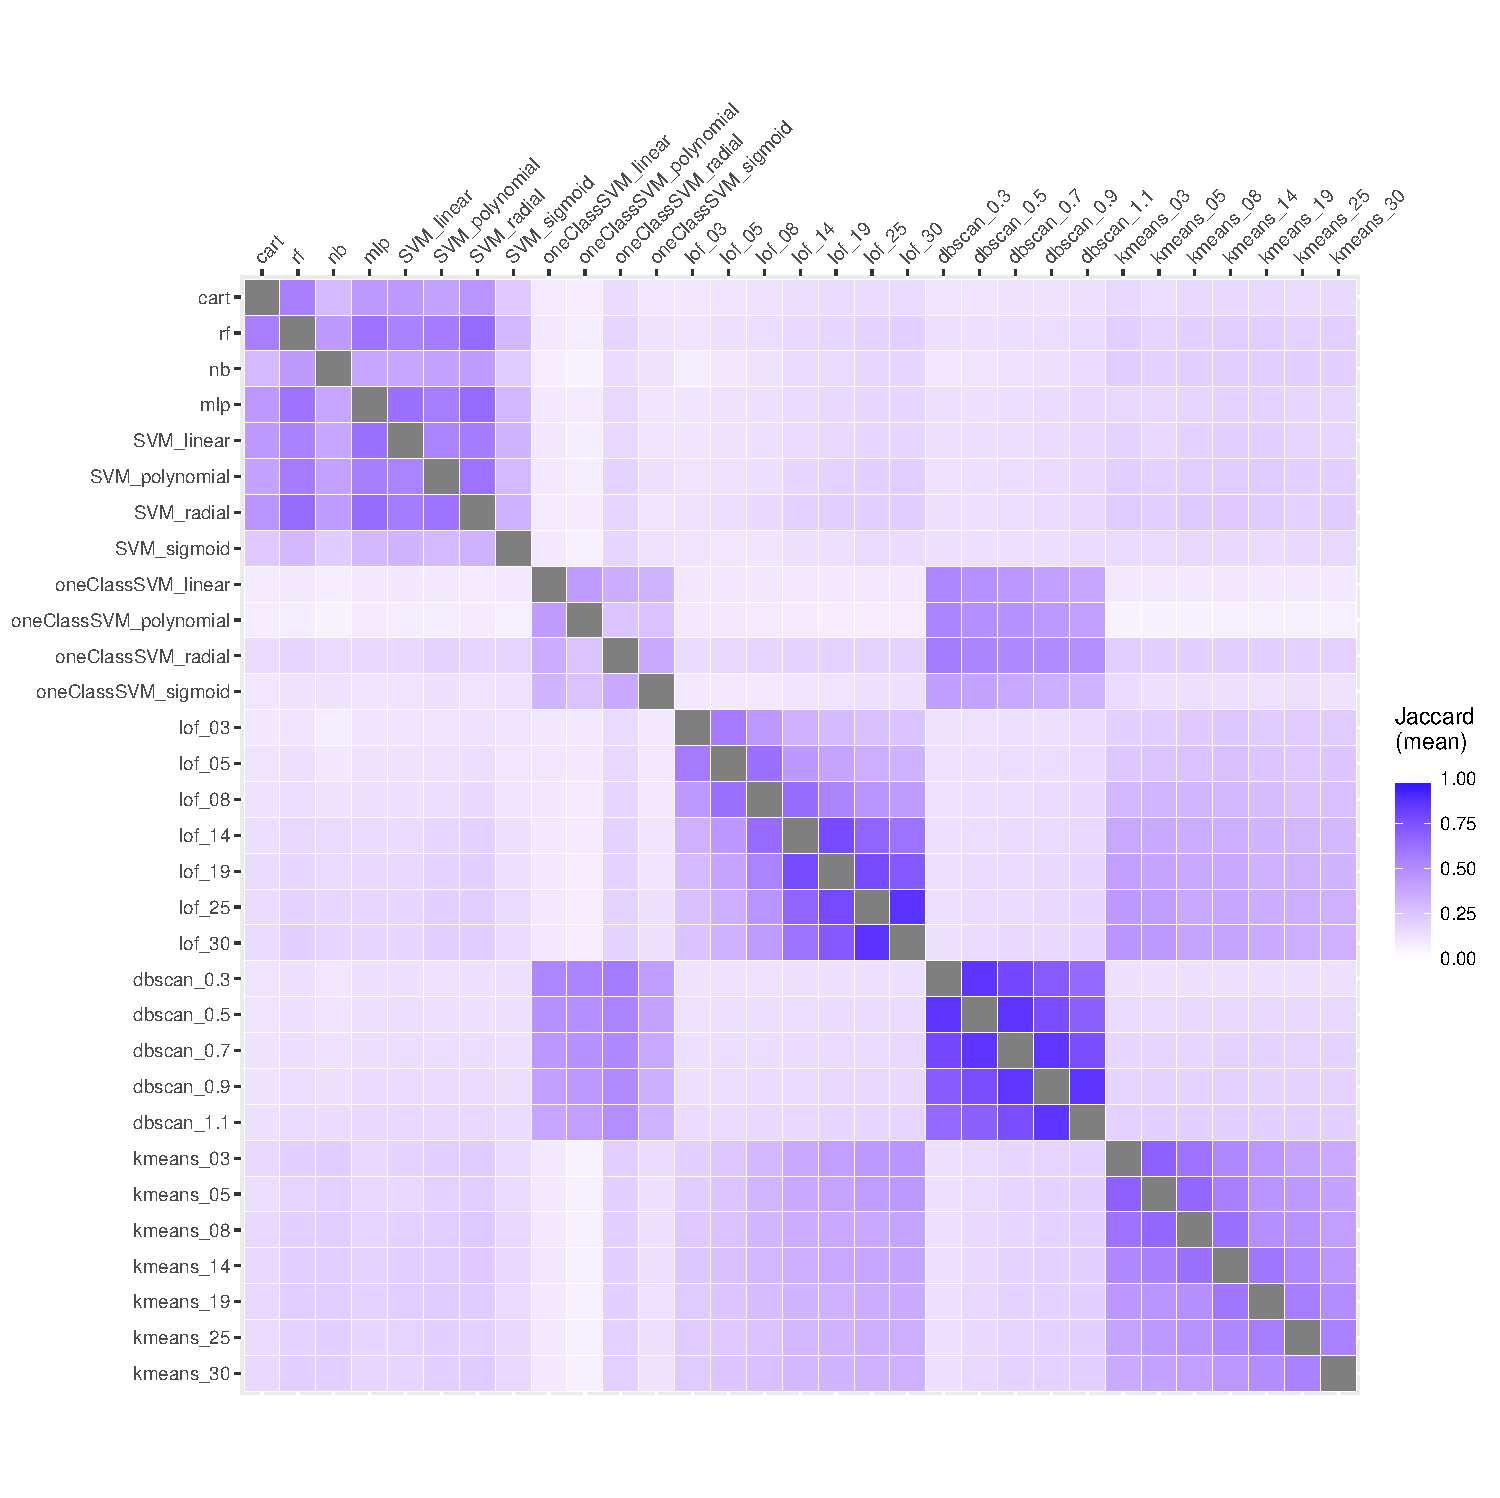
\includegraphics[width=\textwidth]{figures/plot_mean.pdf}
	\caption{Mean value across all datasets of the Jaccard metric between each par of techniques.}
	\label{fig:mean}
\end{figure}

Figure~\ref{fig:sd} show a more distinct variation on the similarity between the supervised learning techniques, between the DBSCAN technique's variations and between the DBSCAN's variations and one of the variations of the One-class SVM technique.

\begin{figure}[ht!]
	\centering
	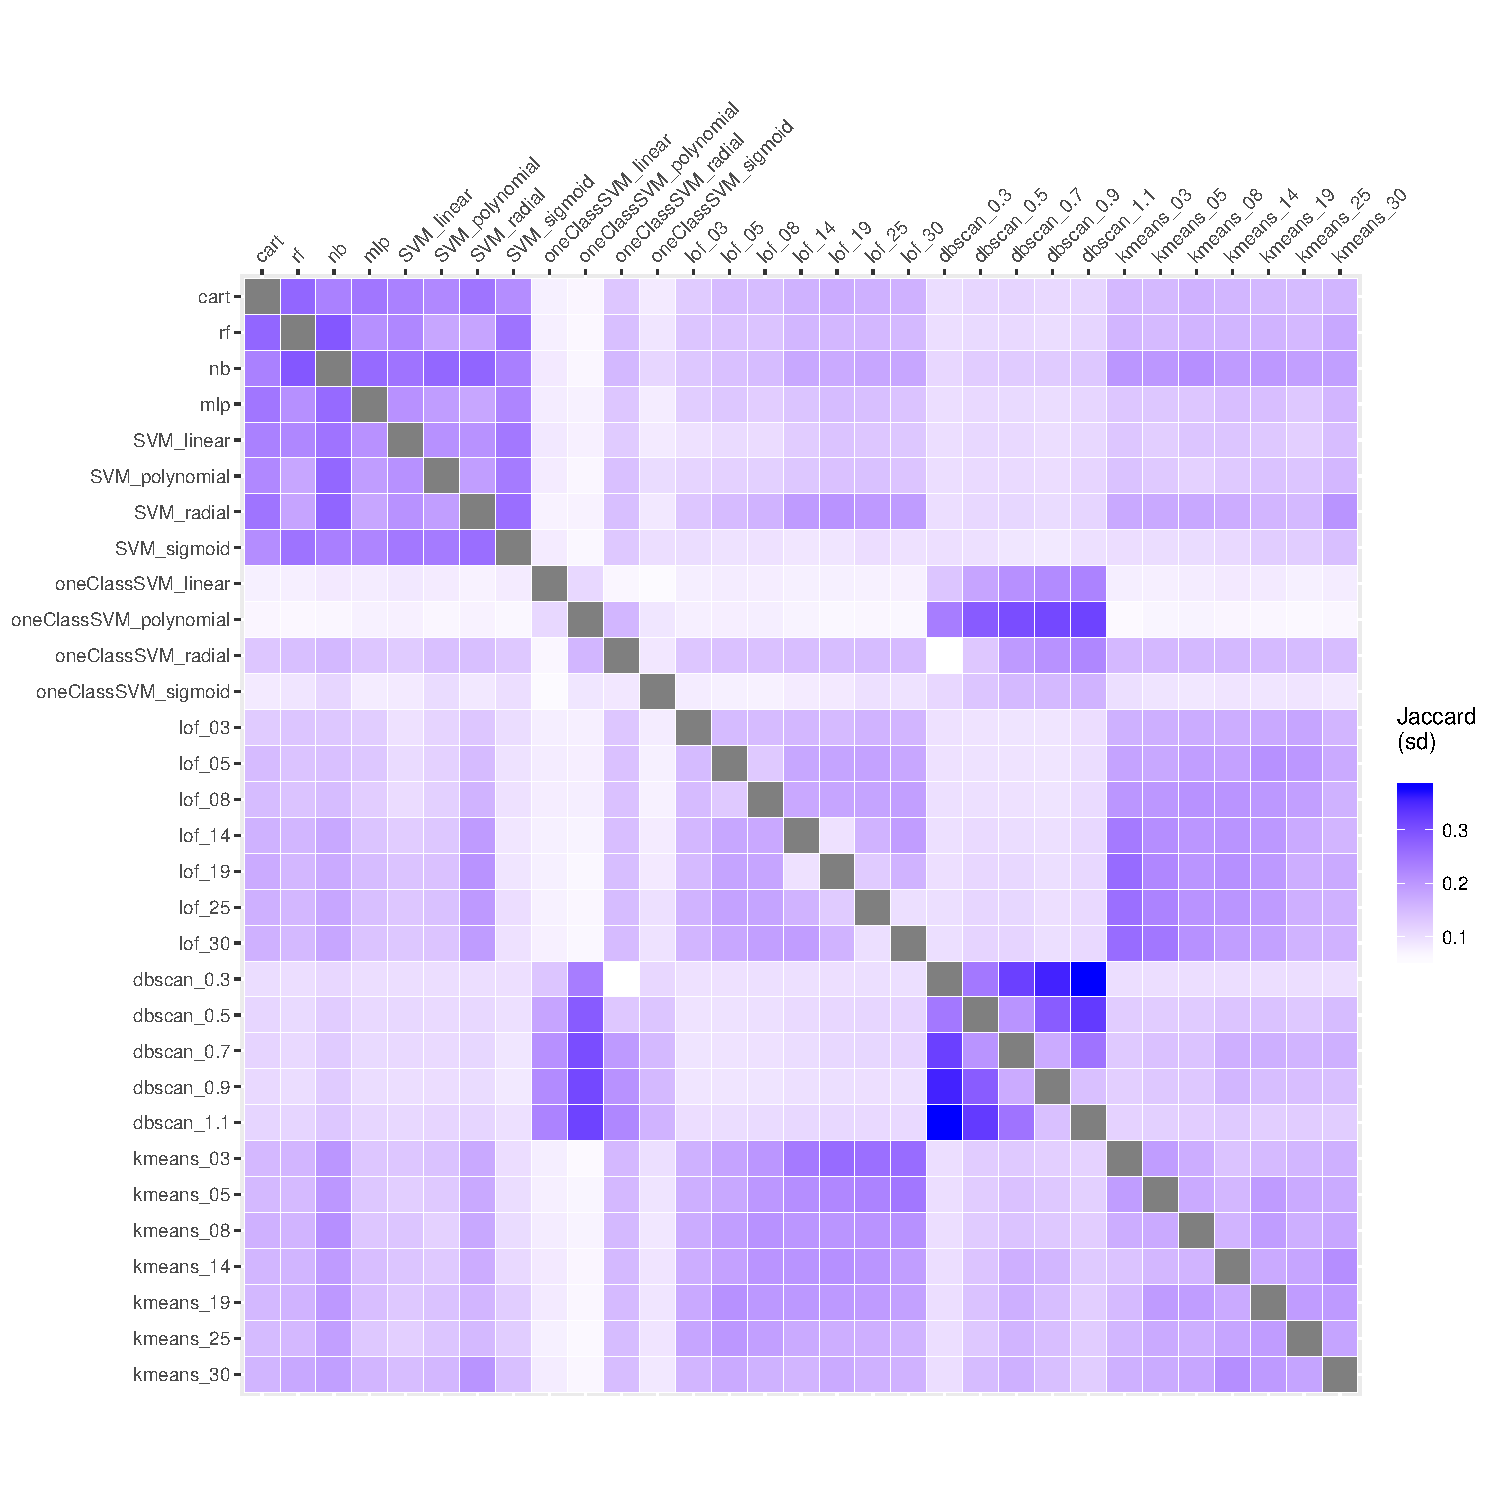
\includegraphics[width=\textwidth]{figures/plot_sd.pdf}
	\caption{Standard deviation value across all datasets of the Jaccard metric between each par of techniques.}
	\label{fig:sd}
\end{figure}

\section{Study on Stacking Approaches}

Table~\ref{tab:stacking_better_no_maj} lists the best Stacking approaches that outperformed the best single technique for each dataset.
In 12 of the 21 datasets there was an improvement in the F1's value over the best technique. The mean improvement in these 12 datasets was 0.025.

Regarding the techniques used in the ensemble, the best ensemble in 6 of the 12 datasets contained techniques from several learning modes: this is the case of the datasets ALOI, KDDCup99, WPBC, InternetAds, PageBlocks and Stamps.
In 5 of these 6 datasets, the best ensemble was the one that included all the techniques.
Given these results, there is not a clear conclusion on whether including techniques from different learning modes results in an ensemble with higher accuracy.

Regarding the best meta-classifier, there was not one that outperformed consistently all the others on the datasets used.

\begin{table}[!ht]
	\centering
	\caption{Measurements of the metric F1 for the Stacking approaches that outperform the best algorithm for each dataset.}
	\label{tab:stacking_better_no_maj}
	\resizebox{\textwidth}{!}{%
		\begin{tabular}{@{}llllll@{}}
			\toprule
			\textbf{Dataset} & \textbf{Ensemble Techniques} & \textbf{Meta-classifier} & \textbf{Best Technique F1} & \textbf{Best Ensemble F1} & \textbf{Improvement} \\ \midrule
			ALOI & All & RF & 0.933 & 0.947 & +0.014 \\
			KDDCup99 & All & RF & 0.852 & 0.879 & +0.027 \\
			Shuttle & One-class SVM + SVM & LR & 0.900 & 1.000 & +0.100 \\
			& One-class SVM + SVM & MLP & 0.900 & 1.000 & +0.100 \\
			& SVM & LR & 0.900 & 1.000 & +0.100 \\
			& SVM & MLP & 0.900 & 1.000 & +0.100 \\
			Waveform & SVM & CART & 0.600 & 0.640 & +0.040 \\
			WPBC & One-class SVM + SVM & MLP & 0.536 & 0.569 & +0.033 \\
			Annthyroid & All Supervised & CART & 0.974 & 0.976 & +0.002 \\
			Cardiotocography & All Supervised & CART & 0.899 & 0.905 & +0.006 \\
			HeartDisease & CART + RF & MLP & 0.650 & 0.672 & +0.022 \\
			InternetAds & All & LR & 0.880 & 0.898 & +0.018 \\
			PageBlocks & All & RF & 0.885 & 0.890 & +0.005 \\
			SpamBase & All Supervised & RF & 0.873 & 0.882 & +0.009 \\
			Stamps & All & CART & 0.886 & 0.906 & +0.020 \\ \bottomrule
	\end{tabular}}
\end{table}

Table~\ref{tab:stacking_better} lists the best Stacking approaches that outperformed the best single technique for each dataset, but this time considering additionally Majority Voting as an alternative to a meta-classifier.
Majority Voting is not a meta-classifier, so therefore a solution with it cannot be considered an application of the Stacking method.
However, the inclusion of Majority Voting can provide insight on whether how well the meta-classifiers are performing, by serving as a baseline.

In this case, in 15 of the 21 datasets there was an improvement of the F1's value over the best technique: more 3 datasets than without considering Majority Voting.
The mean value of this improvement was 0.056, also higher than the one from the previous experiment. The techniques included in most of the successful ensembles are the RF and CART algorithms, with Majority Voting being a better alternative to a meta-classifier in all datasets except Waveform and Stamps.

%Table~\ref{tab:stacking_better} lists the best Stacking approaches that outperformed the best single technique for each dataset. 
%The stacking approach outperformed the best individual technique in 15 of the 21 datasets, with the combination of the CART and Random Forest techniques as an ensemble and Majority Voting as a meta-classifier the most frequent combination (in 10 of the datasets).
%In most of the datasets, an ensemble of supervised learning techniques always outperformed an ensemble with techniques from several learning modes.
%Regarding the improvement observed, Stacking had a mean improvement of 0.0671 in the F1 metric's value

\begin{table}[!ht]
	\centering
	\caption{Measurements of the metric F1 for the Stacking approaches that outperform the best algorithm for each dataset, when considering Majority Voting as an alternative to a meta-classifier.}
	\label{tab:stacking_better}
	\resizebox{\textwidth}{!}{%
\begin{tabular}{@{}llllll@{}}
	\toprule
	\textbf{Dataset} & \textbf{Ensemble Techniques} & \textbf{Meta-classifier} & \textbf{Best Technique F1} & \textbf{Best Ensemble F1} & \textbf{Improvement} \\ \midrule
	ALOI & CART + RF & Majority Voting & 0.590 & 0.742 & +0.152 \\
	Ionosphere & DBSCAN & Majority Voting & 0.933 & 1.000 & +0.067 \\
	KDDCup99 & CART + RF & Majority Voting & 0.852 & 0.892 & +0.040 \\
	Shuttle & All Supervised & Majority Voting & 0.900 & 1.000 & +0.100 \\
	 & One-class SVM + SVM & LR & 0.900 & 1.000 & +0.100 \\
	 & One-class SVM + SVM & MLP & 0.900 & 1.000 & +0.100 \\
	 & SVM & Majority Voting & 0.900 & 1.000 & +0.100 \\
	 & SVM & LR & 0.900 & 1.000 & +0.100 \\
	 & SVM & MLP & 0.900 & 1.000 & +0.100 \\
	Waveform & SVM & CART & 0.600 & 0.640 & +0.040 \\
	WPBC & CART + RF & Majority Voting & 0.536 & 0.625 & +0.089 \\
	Annthyroid & CART + RF & Majority Voting & 0.974 & 0.979 & +0.005 \\
	Arrhythmia & CART + RF & Majority Voting & 0.587 & 0.653 & +0.066 \\
	Cardiotocography & CART + RF & Majority Voting & 0.899 & 0.928 & +0.029 \\
	HeartDisease & CART + RF & Majority Voting & 0.650 & 0.676 & +0.026 \\
	InternetAds & All Supervised & Majority Voting & 0.880 & 0.913 & +0.032 \\
	PageBlocks & CART + RF & Majority Voting & 0.885 & 0.919 & +0.034 \\
	Pima & CART + RF & Majority Voting & 0.541 & 0.647 & +0.106 \\
	SpamBase & CART + RF & Majority Voting & 0.873 & 0.908 & +0.036 \\
	Stamps & All & CART & 0.886 & 0.906 & +0.020 \\ \bottomrule
\end{tabular}}
\end{table}

%It might be somewhat debatable if the Majority Voting can be considered a simpler Stacking approach. Therefore, the results of this study without the Majority Voting algorithm being considered as a meta-classifier are displayed in table~\ref{tab:stacking_better_no_maj}
%In this case, in 12 of the 21 datasets there was an improvement in the F1's value over the best technique.
%Regarding the techniques used in the ensemble, once again there was no benefit in using \textit{hybrid} ensemble with techniques from several learning modes.


\chapter{Conclusions and Future Work} \label{chap:conc}

\section*{}

This chapter presents the main conclusions of this research work in the context of Anomaly Detection and Ensemble Learning and possible future work topics.

\section{Main Overview and Conclusions}

On this dissertation, we first discussed the concepts of Anomaly Detection and Ensemble Learning. A taxonomy and applications for both of the fields was also presented, among with a definition of the Stacked Generalization method and its applications in the Anomaly Detection context.

We then proposed an experimental methodology, separated in two experimental studies, to tackle the application the Stacked Generalization method in the context of Anomaly Detection.
Several Anomaly Detection techniques from different taxonomic groups were studied separately and combined with different meta-classifiers.
These studies were supported by datasets used throughout the literature of Anomaly Detection.
The main results and findings of this experimental methodology were also exposed.

We can briefly summarize the main conclusions of this dissertation as follows:

\begin{itemize}
	
	\item Most of the Anomaly Detection techniques used in this study are \textit{accurate} and \textit{diverse} in the datasets used, therefore having the necessary conditions for the Stacking method over-performing the best technique in each dataset.
	\item The application of the Stacking method guaranteed higher F1 values than the best Anomaly Detection technique on more than half of the datasets used.
	\item There is no clear indication whether including Anomaly Detection techniques from different learning modes guarantees higher F1 values. In the datasets where this was true, the best combination was including techniques from all the learning modes available.
	\item There is not a meta-classifier that clearly outperformed the others in terms of F1 on the datasets, so choosing the appropriate one seems to be very dependent on the dataset.
	\item Replacing the meta-classifier with the Majority Voting method improved the F1 value on even more datasets, with also a higher mean improvement on the F1. In this case, ensembles with tree-based Anomaly Detection techniques only (CART and Random Forest) were the ones with higher F1 values on most datasets.
	%\item The best approach in combining Anomaly Detection with best performance on the tested datasets is by combining the \textit{opinions} of two tree-based supervised algorithms (CART and Random Forest) with a Majority Voting meta-classifier;
	%\item In most of the datasets, there was no advantage in terms of performance in including in an ensemble supervised and unsupervised learning Anomaly Detection techniques, as ensembles of supervised learning techniques reveled to be the most promising.
\end{itemize}

\section{Main Contributions}

The main contribution of this dissertation is the the development of a research study on Stacking approaches applied to Anomaly Detection with a broader variety of techniques, meta-classifiers and datasets.
Also a study on the performance and diversity of these techniques across datasets used throughout the Anomaly Detection literature was also provided as a secondary contribution.

%The main contributions of this dissertation can be summarized as follows:

%\begin{itemize}
%	\item Development of a research study on Stacking approaches applied to Anomaly Detection with a broader variety of techniques meta-classifiers;
%	\item 
%\end{itemize}

\section{Future Work}

Several ideas can be followed as future work to the research work developed in this dissertation:

\begin{itemize}
	\item \textit{Bigger datasets}: One of the limitations of the experimental methodology proposed was the size of the datasets used. Although from our point of view it is important to perform a study on datasets that were used previously in the literature in order to enable further comparisons, these datasets are in general very small.
	More complex methodologies with processes like parameter optimization would need bigger datasets in order to perform validation in a greater number of data instances.
	\item \textit{Higher variety of Anomaly Detection techniques}: Although this dissertation performed an empirical evaluation on Stacking with a greater variety of Anomaly Detection techniques than previous studies (at least, to the best of our knowledge), more techniques could be incorporated and tested.
	In particular, there were taxonomic groups of Anomaly Detection techniques that were not explored, mostly because the application of these techniques is not as popular, and therefore there is a lack of implementations in general purpose languages.
	Therefore, the exploration of this future work idea most probably implicate some implementation work.
\end{itemize}

%%----------------------------------------
%% Final materials
%%----------------------------------------

%% Bibliography
%% Comment the next command if BibTeX file not used
%% bibliography is in ``myrefs.bib''
%\PrintBib{myrefs}
\PrintBibliographyBiblatex

%% comment next 2 commands if numbered appendices are not used
\appendix
%\chapter{Loren Ipsum} \label{ap1:loren}

Depois das conclusões e antes das referências bibliográficas,
apresenta-se neste anexo numerado o texto usado para preencher a
dissertação.

\section{O que é o \emph{Loren Ipsum}?}

\emph{\textbf{Lorem Ipsum}} is simply dummy text of the printing and
typesetting industry. Lorem Ipsum has been the industry's standard
dummy text ever since the 1500s, when an unknown printer took a galley
of type and scrambled it to make a type specimen book. It has survived
not only five centuries, but also the leap into electronic
typesetting, remaining essentially unchanged. It was popularised in
the 1960s with the release of Letraset sheets containing Lorem Ipsum
passages, and more recently with desktop publishing software like
Aldus PageMaker including versions of Lorem Ipsum. 

\section{De onde Vem o Loren?}

Contrary to popular belief, Lorem Ipsum is not simply random text. It
has roots in a piece of classical Latin literature from 45 BC, making
it over 2000 years old. Richard McClintock, a Latin professor at
Hampden-Sydney College in Virginia, looked up one of the more obscure
Latin words, consectetur, from a Lorem Ipsum passage, and going
through the cites of the word in classical literature, discovered the
undoubtable source. Lorem Ipsum comes from sections 1.10.32 and
1.10.33 of ``de Finibus Bonorum et Malorum'' (The Extremes of Good and
Evil) by Cicero, written in 45 BC. This book is a treatise on the
theory of ethics, very popular during the Renaissance. The first line
of Lorem Ipsum, ``Lorem ipsum dolor sit amet\ldots'', comes from a line in
section 1.10.32.

The standard chunk of Lorem Ipsum used since the 1500s is reproduced
below for those interested. Sections 1.10.32 and 1.10.33 from ``de
Finibus Bonorum et Malorum'' by Cicero are also reproduced in their
exact original form, accompanied by English versions from the 1914
translation by H. Rackham.

\section{Porque se usa o Loren?}

It is a long established fact that a reader will be distracted by the
readable content of a page when looking at its layout. The point of
using Lorem Ipsum is that it has a more-or-less normal distribution of
letters, as opposed to using ``Content here, content here'', making it
look like readable English. Many desktop publishing packages and web
page editors now use Lorem Ipsum as their default model text, and a
search for ``lorem ipsum'' will uncover many web sites still in their
infancy. Various versions have evolved over the years, sometimes by
accident, sometimes on purpose (injected humour and the like). 

\section{Onde se Podem Encontrar Exemplos?}

There are many variations of passages of Lorem Ipsum available, but
the majority have suffered alteration in some form, by injected
humour, or randomised words which don't look even slightly
believable. If you are going to use a passage of Lorem Ipsum, you need
to be sure there isn't anything embarrassing hidden in the middle of
text. All the Lorem Ipsum generators on the Internet tend to repeat
predefined chunks as necessary, making this the first true generator
on the Internet. It uses a dictionary of over 200 Latin words,
combined with a handful of model sentence structures, to generate
Lorem Ipsum which looks reasonable. The generated Lorem Ipsum is
therefore always free from repetition, injected humour, or
non-characteristic words etc. 


%% Index
%% Uncomment next command if index is required
%% don't forget to run ``makeindex mieic-en'' command
%\PrintIndex

\end{document}
